\documentclass{beamer}
\usepackage[utf8]{inputenc}

\usetheme{Madrid}
\usecolortheme{default}

%------------------------------------------------------------
% Title Page Configuration
%------------------------------------------------------------
\title[Agent-Based Crowd Simulation]
{Agent-Based Crowd Simulation for Stampede Prevention and Event Safety}

\subtitle{Final Review}

\author[Group 13] 
{
    \textbf{Project Team:}\\
    Nivin P Louis (TL23BTAI0042)\\
    Niranjana Sreevalsan (TL23BTAI0348)\\
    Farhan Mohamed T P (TL23BTAI0308)\\
    Nihal Shakheer (TL23BTAI0249)\\[0.5cm]
    \textbf{Project Guide:}\\
    Anju K P, Assistant Professor, Dept. AIML
}

\institute[Dept. AIML] 
{
    Vidya Academy of Science and Technology, Thrissur
}

\date[\today]

%------------------------------------------------------------
% Table of Contents Configuration
%------------------------------------------------------------

\begin{document}

%---------------------------------------------------------
% Slide 1: Title
%---------------------------------------------------------
\frame{\titlepage}

% Slide 2: Vision and Mission
\begin{frame}
\centering

\footnotesize  % body text size (kept small to fit)

% Logo

\includegraphics[width=0.26\textwidth]{college_logo.png}

\vspace{0.25cm}

% ---- College Vision ----
{\normalsize\bfseries College Vision}\\
Progress through education

\vspace{0.25cm}

% ---- College Mission ----
{\normalsize\bfseries College Mission}\\
To seek, strive for and scale greater heights of quality education

\vspace{0.3cm}

% ---- Department Vision ----
{\normalsize\bfseries Department Vision}\\
To evolve as a center of excellence for higher education in the field of
Artificial Intelligence and Machine Learning

\vspace{0.3cm}

% ---- Department Mission ----
{\normalsize\bfseries Department Mission}

\vspace{0.15cm}

M1: To equip graduates with the latest technologies in Artificial Intelligence and Machine Learning

\vspace{0.1cm}

M2: To imbibe new knowledge by collaborating with industry and research organizations to mould competent technocrats and entrepreneurs

\vspace{0.1cm}

M3: To instill societal and ethical responsibilities in all professional activities

\end{frame}
 
%---------------------------------------------------------
% Slide 2: Index
%---------------------------------------------------------
\begin{frame}
\frametitle{Index}
\tableofcontents
\end{frame}

%---------------------------------------------------------
% Section: Motivation
%---------------------------------------------------------
\section{Motivation}

\begin{frame}
\frametitle{Motivation}
\footnotesize % Reducing font size to fit full text


\begin{itemize}
    \item \textbf{Critical Safety Risks:} Large-scale gatherings are increasingly prone to dangerous overcrowding and stampedes, often caused by inadequate infrastructure planning rather than the crowd itself.
    \item \textbf{Limitations of Traditional Models:} Standard "fluid-based" models treat crowds as a homogeneous mass, failing to capture the complex, individual decision-making (micro-interactions) that leads to disasters.
    \item \textbf{Emergent Behavior Complexity:} Dangerous phenomena like "contagious panic" and crushing pressures arise from individual interactions that are difficult to predict without granular simulation.
    \item \textbf{Cost of Trial and Error:} Testing crowd control measures in real-world scenarios is dangerous and impossible; a virtual environment is required to safely test "what-if" emergency scenarios.
    \item \textbf{Need for Dynamic Layout Analysis:} Static capacity calculations cannot account for dynamic bottlenecks (e.g., security checks, narrow gates) where flow rates fluctuate rapidly.
\end{itemize}
\end{frame}

%---------------------------------------------------------
% Section: Objective
%---------------------------------------------------------
\section{Objective}

\begin{frame}
\frametitle{Objective}
\footnotesize 


\begin{itemize}
    \item \textbf{Develop an Agent-Based Model (ABM):} Create a simulation where every individual is modeled as an autonomous agent with specific goals, local perception, and collision avoidance rules.
    \item \textbf{Simulate Realistic Crowd Psychology:} Implement parameters for "panic propagation" and agent pressure to model how calm movement transitions into aggressive pushing or irrational behavior.
    \item \textbf{Model Complex Environments:} Build a flexible environment system that accounts for physical constraints, such as obstacles, one-way paths, and varying exit widths.
    \item \textbf{Visualize Risk Zones:} Generate real-time analytics, including density heatmaps and congestion maps, to automatically identify potential crush zones before they occur.
    \item \textbf{Evaluate Intervention Strategies:} Quantify the safety impact of specific protocols, such as optimizing exit placement or introducing "cooperative agents" to guide crowds during evacuations.
\end{itemize}
\end{frame}

%---------------------------------------------------------
% Section: Literature Review
%---------------------------------------------------------
\section{Literature Review}

% --- Paper 1 ---
\begin{frame}
\frametitle{Literature Review\newline Paper 1: Enhancing Building Evacuation Efficiency}
\framesubtitle{in Case of Fire Breakout by Integrating Evacuee Categorization Into an Agent-Based Simulation (Vol. 17, January 2025)}
\scriptsize

\begin{block}{Objective}
To develop an agent-based model that enhances building evacuation efficiency during fire breakouts, by categorizing evacuees based on their health status and familiarity with the layout to assign tailored evacuation strategies.
\end{block}



\textbf{Methodology}
\begin{enumerate}
    \item \textbf{Agent-Based Modeling Framework:} To simulate autonomous interactions between various entities—including people, fire, smoke, and obstacles—within a hospital environment.
    \item \textbf{Agent Categorization:} Based on their health status (healthy vs. sick) and familiarity with the building layout, utilizing a three-layer behavioral architecture (planning, searching for an exit, and collision avoidance).
    \item \textbf{Scenario-Based Simulation and Analysis:} Varying factors such as fire positioning, population density, and the addition of emergency exits—using distinct algorithms to measure survival rates and evacuation times.
\end{enumerate}
\end{frame}

\begin{frame}
\frametitle{Paper 1: Results \& Conclusion}
\scriptsize

\textbf{Results / Key Findings}
\begin{itemize}
    \item \textbf{Impact of Knowledge and Health Status:} Agents familiar with the building layout, particularly those employing wall-following algorithms during low visibility, evacuate significantly faster with fewer fatalities, whereas sick or unfamiliar agents face higher mortality rates due to disorientation and physical limitations.
    \item \textbf{Structural Optimizations:} Addition of transverse doors and emergency exits in high-density areas (such as delivery rooms) drastically improves survival rates by alleviating congestion at main exits and reducing the travel distance required to escape.
    \item \textbf{Fire Positioning and Density Effects:} High population density and central fire locations create severe bottlenecks that trap occupants and increase evacuation times, whereas decentralized fires allow for more effective use of available exits.
\end{itemize}

\begin{alertblock}{Conclusion}
Integrating evacuee categorization based on health status and spatial familiarity into an agent-based model, combined with strategic architectural improvements like additional emergency exits, significantly enhances hospital evacuation efficiency and reduces mortality rates during fire emergencies.
\end{alertblock}
\end{frame}

% --- Paper 2 ---
\begin{frame}
\frametitle{Literature Review\newline Paper 2: RESCUE: Crowd Evacuation Simulation}
\framesubtitle{via Controlling SDM-United Characters (October 2025)}
\scriptsize

\begin{block}{Objective}
To develop an online, physically realistic 3D crowd evacuation simulation framework called RESCUE that utilizes a neuroscience-inspired sensory-decision-motor loop to generate personalized, adaptive agent behaviors and complex interactions across varying terrains.
\end{block}



\textbf{Methodology}
\begin{itemize}
    \item \textbf{SDM-United Framework:} The methodology creates a continuous Sensory-Decision-Motor (SDM) loop where agents perceive their self-state and environment, calculate navigation strategies, and execute physical movements, simulating the human brain's processing flow.
    \item \textbf{Social Force Modelling:} To navigate complex environments, that incorporates specific "evasive forces" to prevent falls and collisions, while applying personalized coefficients to adjust speeds based on individual attributes like age or physical disability.
    \item \textbf{Personalized Gait Motor:} Employs a diffusion-based Personalized Gait Controller that transforms standard path-following actions into diverse, physically realistic gaits, enabling agents to maintain balance on uneven terrain while exhibiting distinct movement styles.
\end{itemize}
\end{frame}

\begin{frame}
\frametitle{Paper 2: Results \& Conclusion}
\scriptsize

\textbf{Results / Key Findings}
\begin{itemize}
    \item \textbf{Superior Simulation Performance:} The RESCUE framework significantly outperforms state-of-the-art methods like OmniControl and MaskedMimic, achieving a higher average escape success rate (0.84) and fewer falls (12.26) by effectively balancing pathfinding with collision avoidance.
    \item \textbf{3D Realism:} The system successfully generates diverse, physically plausible motions where agents exhibit distinct speeds and gaits tailored to individual attributes (e.g., age, disability), overcoming the uniformity and lack of physical realism found in traditional models.
    \item \textbf{Environmental Adaptability:} The framework adapts to complex environmental factors—such as uneven terrain, slippery surfaces, and bottlenecks—to realistically simulate hazards like trampling, part-level force visualization to precisely analyze contact forces and potential injuries.
\end{itemize}

\begin{alertblock}{Conclusion}
The proposed RESCUE framework successfully leverages a neuroscience-inspired sensory-decision-motor loop to deliver superior, physically realistic, and personalized 3D crowd evacuation simulations that offer critical insights for enhancing public safety.
\end{alertblock}
\end{frame}

% --- Paper 3 ---
\begin{frame}
\frametitle{Literature Review\newline Paper 3: Modelling Mass Crowd Using Discrete Event}
\framesubtitle{Simulation: A Case Study of Integrated Tawaf and Sayee Rituals During Hajj (Vol. 7,June 2021)}
\scriptsize

\begin{block}{Objective}
The objective of this research is to simulate and validate real Hajj data using Discrete Event Simulation to model the integrated Tawaf and Sayee rituals under normal and evacuation conditions, allowing for the assessment of capacity and behavioral contributions to congestion and the evaluation of crowd management strategies within the Grand Mosque.
\end{block}



\textbf{Methodology}
\begin{enumerate}
    \item \textbf{Integrated Discrete Event Simulation (DES) Framework:} Specifically the ExtendSim software, to build a macro-level model that integrates both Tawaf and Sayee rituals into a single system. Unlike previous studies that modeled these rituals separately, this approach simulates the continuous flow of pilgrims between the two sites under both normal operating conditions and emergency evacuation situations.
    \item \textbf{Data-Driven Model Construction and Calibration:} Using secondary data from Saudi Hajj authorities, including video analysis from 2015–2017, operational planning documents, and social media reports.
    \item \textbf{Statistical Validation and Sensitivity Analysis:} The model was validated against real-world data from 2015 to 2019 using statistical methods to ensure accuracy in representing pilgrim flows. The researchers ran the simulation 30 times across over 200 distinct scenarios
\end{enumerate}
\end{frame}

\begin{frame}
\frametitle{Literature Review\newline Paper 3: Results \& Conclusion}
\scriptsize

\textbf{Results / Key Findings}
\begin{itemize}
    \item \textbf{Critical Capacity and Bottlenecks:} The simulation identified the main Tawaf area and Sayee Ground Level as the most critical bottlenecks, reaching densities of 6 pilgrims/m², yet revealed the infrastructure has reserve capacity to potentially accommodate up to 4 million pilgrims.
    \item \textbf{Strategic Flow Management:} Assigning specific entry gates to pilgrim groups reduced the total time to complete rituals by over two hours.
    \item \textbf{Efficient Evacuation Performance:} Demonstrated faster clearance times than previous studies—ranging from approximately 4 to 16 minutes depending on the level—while maintaining safe crowd densities (maximum 3.41 pilgrims/m²) by dynamically utilizing all 179 available gates.
\end{itemize}

\begin{alertblock}{Conclusion}
Researchers created a virtual environment to test how different "shapes" of crowds and "winds" of emergency scenarios interact with the Grand Mosque's architecture, allowing them to spot invisible friction points without risking safety in the real world.
\end{alertblock}
\end{frame}

% --- Paper 4 ---
\begin{frame}
\frametitle{Literature Review\newline Paper 4: Estimate Crowd Flow Including Side-Trip}
\framesubtitle{Behavior When Exiting From Large-Scale Event Venues (Vol. 5, September 2025)}
\scriptsize

\begin{block}{Objective}
To accurately estimate crowd flow in large-scale environments during unforced exit scenarios by developing a simulation model that incorporates stochastic side-trip behaviors.
\end{block}



\textbf{Methodology}
\begin{itemize}
    \item \textbf{Extended Simulation Modeling:} Utilized "CrowdWalk," a multi-agent simulator, and extended it to incorporate stochastic side-trip behaviors. This extension introduces specific parameters to determine the probability (Rst), location (Wst), and duration (tst) of intermediate stops, such as using restrooms, before agents proceed to their final destination.
    \item \textbf{Data Assimilation via Optimization:} Calibrates the model parameters by minimizing the error between the simulated crowd flow and the ground truth data measured at the venue's gates.
    \item \textbf{Real-World Validation and Comparison:} The method was validated using empirical data collected at the Tokyo Dome, where spectator departure times were tracked with 8K cameras and crowd flow was measured using LiDAR sensors. The performance of the proposed side-trip model was statistically compared against traditional shortest-path and gate-selection models to verify improvements in estimation accuracy.
\end{itemize}
\end{frame}

\begin{frame}
\frametitle{Paper 4: Results \& Conclusion}
\scriptsize

\textbf{Results / Key Findings}
\begin{itemize}
    \item \textbf{Significant Accuracy Improvement:} The proposed side-trip model achieved a 9.25\% improvement in simulation accuracy compared to previously established models (such as the shortest-path and gate-selection models) when evaluated using crowd data from the same day.
    \item \textbf{Robust Generalizability:} The method demonstrated strong robustness by maintaining a 3.15\% performance improvement, indicating that the model does not overfit to specific events.
    \item \textbf{Superior Reproduction of Delays:} Statistical analysis confirmed the model was significantly superior to others, as it accurately reproduced the crowd stagnation and delays caused by intermediate stops (like restroom usage) that traditional models failed to capture during peak exit times.
\end{itemize}

\begin{alertblock}{Conclusion}
Think of the results like predicting a road trip arrival time. While the old models only calculated the driving distance and speed limit, this new model accurately predicts the arrival time by also accounting for the likelihood of passengers stopping for snacks or restroom breaks.
\end{alertblock}
\end{frame}

% --- Paper 5 ---
\begin{frame}
\frametitle{Literature Review\newline Paper 5: Towards an IICM}
\framesubtitle{Integrated Intelligent Framework for Crowd Control and Management (Vol. 8, April 2025)}
\scriptsize

\begin{block}{Objective}
To design the Integrated Intelligent Crowd Control and Management (IICCM) framework, which leverages Computer Vision, Artificial Intelligence, and Internet of Things technologies to enhance participant safety and optimize management in large-scale gatherings, specifically utilizing the Hajj pilgrimage as a rigorous test case.
\end{block}



\textbf{Methodology}
\begin{enumerate}
    \item \textbf{Framework Integration:} The research designs the IICM Framework, which unifies four distinct components—Crowd Vision, Crowd e-Health and IoT, Crowd Evacuation, and Cloud-IoT reliability—into a cohesive system for monitoring and managing large-scale gatherings.
    \item \textbf{Advanced AI \& IoT Utilization:} Specifically utilizing Generative Adversarial Networks (GANs) to synthesize training data for rare events and Vision Transformers (ViTs) for accurate identification and tracking, alongside IoT sensors to collect real-time health and environmental data.
    \item \textbf{Implementation:} The system is developed using Python in the Google Colaboratory environment to leverage high-performance GPUs for processing massive video streams, using the Hajj pilgrimage as a rigorous, high-density test case to validate the framework's scalability and robustness.
\end{enumerate}
\end{frame}

\begin{frame}
\frametitle{Paper 5: Results \& Conclusion}
\scriptsize

\textbf{Results / Key Findings}
\begin{itemize}
    \item \textbf{Creation of a Unified Framework:} The primary result is the design of the Integrated Intelligent Crowd Control and Management (IICCM) framework, which successfully integrates typically isolated tasks—crowd vision, e-health, evacuation, and cloud reliability—into a single, cohesive system for the first time.
    \item \textbf{Application of Advanced AI \& IoT:} The research establishes the effectiveness of using Generative Adversarial Networks (GANs) to synthesize training data for rare events (like fires or abnormal behaviors) and Vision Transformers (ViTs) for precise tracking, combined with IoT sensors to monitor real-time health and crowd flow.
    \item \textbf{Scalability and Robustness Validation:} The study identifies the Hajj pilgrimage as the ultimate stress test, demonstrating that the framework’s ability to handle millions of diverse participants confirms its scalability and adaptability for other global large-scale events.
\end{itemize}

\begin{alertblock}{Conclusion}
The Integrated Intelligent Crowd Control and Management (IICCM) framework demonstrates that integrating AI, CV, and IoT technologies to manage the extreme complexities of the Hajj pilgrimage establishes a scalable, robust model applicable to enhancing safety and efficiency at large-scale gatherings worldwide.
\end{alertblock}
\end{frame}

%---------------------------------------------------------
% Section: Comparative Analysis
%---------------------------------------------------------
\section{Comparative Analysis}
\begin{frame}
\frametitle{Comparative Analysis}
\frametitle{Comparative Analysis}
\begin{table}[htbp]
\centering
\tiny                             % very small font for PPT fitting
\setlength{\tabcolsep}{2pt}       % minimal column spacing
\renewcommand{\arraystretch}{0.9} % reduce row height
\caption{Comparative Analysis of Intelligent Crowd Management and Complex Systems}

\begin{tabular}{p{1.1cm} p{1.1cm} p{1.3cm} p{1.0cm} p{1.0cm}}
\hline
\textbf{Paper ID} & \textbf{Objective} & \textbf{Methodology} & \textbf{Tech} & \textbf{Results} \\
\hline
IEEE 10942376 & Integrated Control & Multi-modal Fusion & AI, CV, IoT & Risk Relief \\
IEEE 11123809 & Unforced Flow & Multi-agent Sim & LiDAR, 8K & 9.25\% Gain \\
IEEE 9439797 & Hajj Rituals & DES Modeling & ExtendSim & Bottlenecks \\
IEEE 9826689 & Crowd Health & Sensor Integration & Wearables, LSTM & 92\% Accuracy \\
arXiv:2507.20117 & 3D Evacuation & Brain-inspired SDM & Social Force & Realistic Gait \\
S0951832025 & Reliability & Math Modeling & QRA & Resilience \\
S0960077925 & Vulnerability & DL Dismantling & Graph Theory & Key Nodes \\
IEEE 9834140 & Height Precision & Sparse Signal & MIMO Radar & Multi-level \\
\hline
\end{tabular}

\label{tab1}
\end{table}
\end{frame}


%---------------------------------------------------------
% Section: Architecture
%---------------------------------------------------------
\section{Architecture}
\begin{frame}
\frametitle{Architecture}
    \begin{center}
        % This will fit the image to the text width or 80% of the slide height, 
        % whichever is smaller, so it doesn't get cut off.
        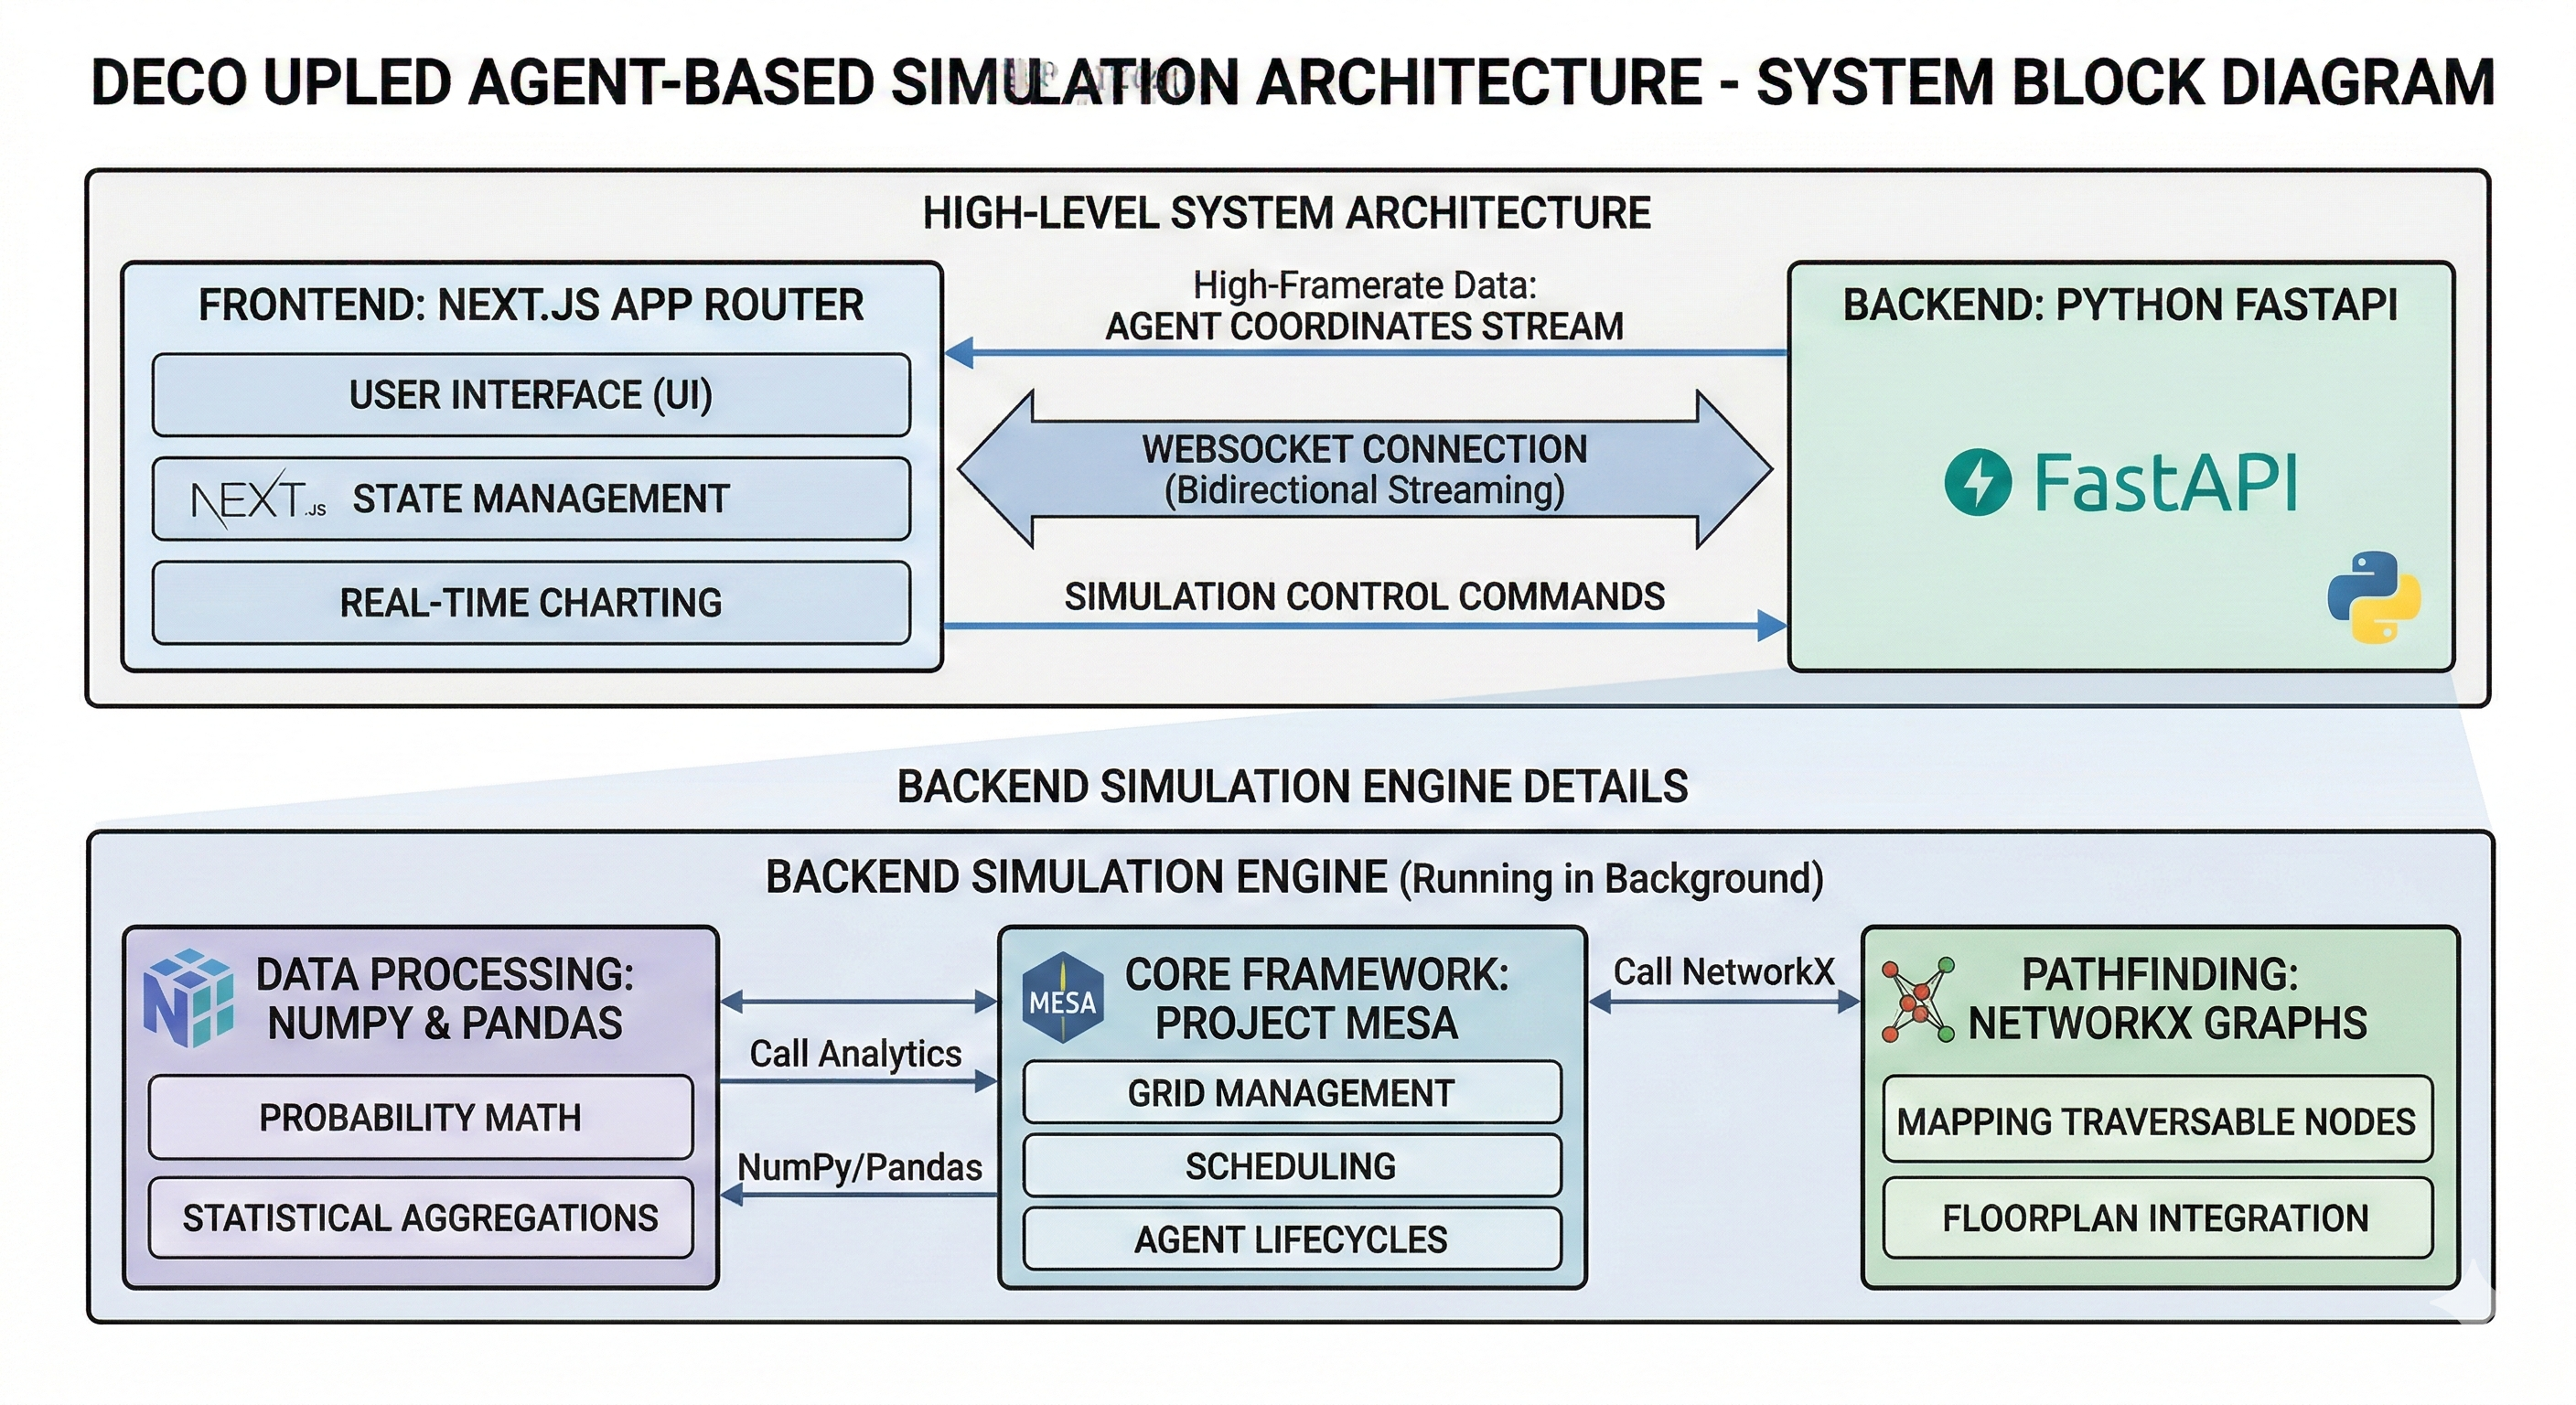
\includegraphics[width=\textwidth, height=0.8\textheight, keepaspectratio]{architecture.png}
    \end{center}
\end{frame}

%---------------------------------------------------------
% Section: Methodology
%---------------------------------------------------------
\section{Methodology}

\begin{frame}
\frametitle{Methodology}
\textbf{Agent-Based Modeling (ABM) Principles} \\
\vspace{0.2cm}
\footnotesize 

\begin{itemize}
    \item \textbf{Core Concept:} Simulating the actions and interactions of autonomous individuals to assess their impact on the overall system (evacuation efficiency).
    \item \textbf{The Agents:} The grid is populated by diverse agents, including Human, Fire, Smoke, Wall, Door, and FireExit.
    \item \textbf{Human States \& Status:} Mobility encompasses Normal, Panic, and Incapacitated states. Overall status tracks whether an agent is Alive, Dead, or Escaped.
    \item \textbf{Health Degradation:} Direct exposure to fire and smoke reduces an agent's health and movement speed. Speed drops significantly when health falls below 50\%.
    \item \textbf{Emergent Collaboration:} Agents dynamically decide to help peers based on an internal "collaboration cost" function, providing Physical Support (carrying), Morale Support (calming), and Verbal Support (sharing exit knowledge).
\end{itemize}
\end{frame}

\begin{frame}
\frametitle{Methodology}
\textbf{Core Algorithms \& Mechanics} \\
\vspace{0.2cm}
\footnotesize 

\begin{itemize}
    \item \textbf{Vision \& Line-of-Sight (Bresenham's Algorithm):} Agents use a CPU-bound ray-tracing method to "see" their surroundings. Sight is strictly blocked by walls and dynamically reduced by accumulating smoke density.
    \item \textbf{Dynamic Pathfinding (NetworkX):} The floorplan is mapped as a graph. Agents calculate the shortest path to an exit or peer in need, executing a retreat and recalculation if fire or smoke is detected on their path.
    \item \textbf{Panic \& Shock Scoring:} Panic is calculated continuously using a mathematical blend of an agent's health, baseline nervousness, experience, and current "shock" (which increases when witnessing fire, smoke, casualties, or panicked peers).
    \item \textbf{Panic Thresholds:} Reaching the panic threshold (0.8) causes agents to forget known floorplan tiles and move erratically, or even faint if panic exceeds 90\%.
\end{itemize}
\end{frame}

%---------------------------------------------------------
% Section: Implementation
%---------------------------------------------------------
\section{Implementation}

\begin{frame}
\frametitle{Implementation}
\textbf{Real-Time State Synchronization} \\
\vspace{0.2cm}
\footnotesize 

\begin{itemize}
    \item \textbf{The WebSocket Pipeline:} Replaced the standard HTTP polling method with a persistent WebSocket connection via FastAPI. The Python backend runs the model.step() loop asynchronously and broadcasts the grid state at high frame rates.
    \item \textbf{Frontend State Management:} A custom React hook (useSimulation.ts) ingests the JSON payload containing the updated coordinates of all agents and current environment variables.
    \item \textbf{Optimized Rendering:} Instead of re-rendering a 50x50 grid of 2,500 HTML elements every tick, the Next.js frontend uses absolute CSS positioning mapped to percentage-based coordinates (widthPct, leftPct).
    \item \textbf{Performance Guarantee:} This guarantees fluid animations and responsiveness across all screen sizes without crashing the browser thread.
\end{itemize}
\end{frame}

\begin{frame}
\frametitle{Implementation}
\textbf{Live Statistics \& Data Collection} \\
\vspace{0.2cm}
\footnotesize 

\begin{itemize}
    \item \textbf{Continuous Metric Aggregation:} The simulation utilizes a data collector to aggregate critical agent metrics on every single step.
    \item \textbf{Survival \& Mobility Tracking:} Real-time counts of agents that are Alive, Dead, or Escaped, along with monitoring how the crowd shifts between Normal, Panic, and Incapacitated states as the fire spreads.
    \item \textbf{Quantifying Emergent Teamwork:} The system tracks specific collaborative actions, including Verbal Collaboration, Physical Collaboration, and Morale Collaboration.
    \item \textbf{Dynamic Visualizations:} The raw data is piped into the Recharts library on the frontend, generating real-time, interactive line graphs that map the trajectory of the evacuation.
\end{itemize}
\end{frame}

%---------------------------------------------------------
% Section: Implementation Overview
%---------------------------------------------------------

\begin{frame}
\frametitle{Implementation}
\textbf{Implementation Overview - Backend (Python / FastAPI)}
\footnotesize 

\begin{itemize}
    \item \textbf{api.py (The Engine Wrapper):} Serves as the FastAPI entry point, managing the persistent WebSocket connection (/ws). Contains the \texttt{get\_grid\_state()} function, which serializes the complex Mesa objects into a lightweight JSON payload of coordinates and statistics.
    \item \textbf{model.py (The World):} The core FireEvacuation class initializes the MultiGrid and reads .txt floorplans into matrix arrays. It also manages the DataCollector and the random scheduling of agent turns.
    \item \textbf{agent.py (The Brains):} Contains the dense logic for Human, Fire, Smoke, and environmental agents. The \texttt{Human.step()} function runs sequentially: checking health, updating the Bresenham line-of-sight, calculating panic, and requesting NetworkX to plot the shortest path to safety.
\end{itemize}
\end{frame}

\begin{frame}
\frametitle{Implementation}
\textbf{Implementation Overview - Frontend (Next.js / React)} \\
\vspace{0.2cm}
\footnotesize 

\begin{itemize}
    \item \textbf{useSimulation.ts (State Management):} A custom React Hook that establishes the WebSocket connection and listens for the \texttt{message} event. It maintains the global \texttt{gameState} (agents array, current step, historical stats) without relying on heavy Redux stores.
    \item \textbf{SimulationGrid.tsx (The Canvas):} Maps the JSON agent array into Next.js \texttt{<Image />} components. Dynamically calculates CSS left, top, width, and height as percentages based on \texttt{grid\_width} and \texttt{grid\_height}, ensuring perfect responsiveness.
    \item \textbf{FloorplanBuilder.tsx (Interactive Tools):} A separate React view featuring a drawable CSS grid, allowing users to paint CellType strings (W, F, D, E) and POST them back to the server as custom .txt files.
    \item \textbf{Charts.tsx \& Controls.tsx (UI/UX):} Modular components parsing the history array into Recharts line graphs and providing sliders/toggles to configure initial simulation constraints.
\end{itemize}
\end{frame}
%---------------------------------------------------------
% Section:   Code Snippets
%---------------------------------------------------------
\section{ \& Code Snippets}

\begin{frame}
\frametitle{Code Snippet}
\footnotesize 

\begin{center}
    \textbf{agent.py} \\
    (Characteristics of various agents) \\
    \vspace{0.2cm}
    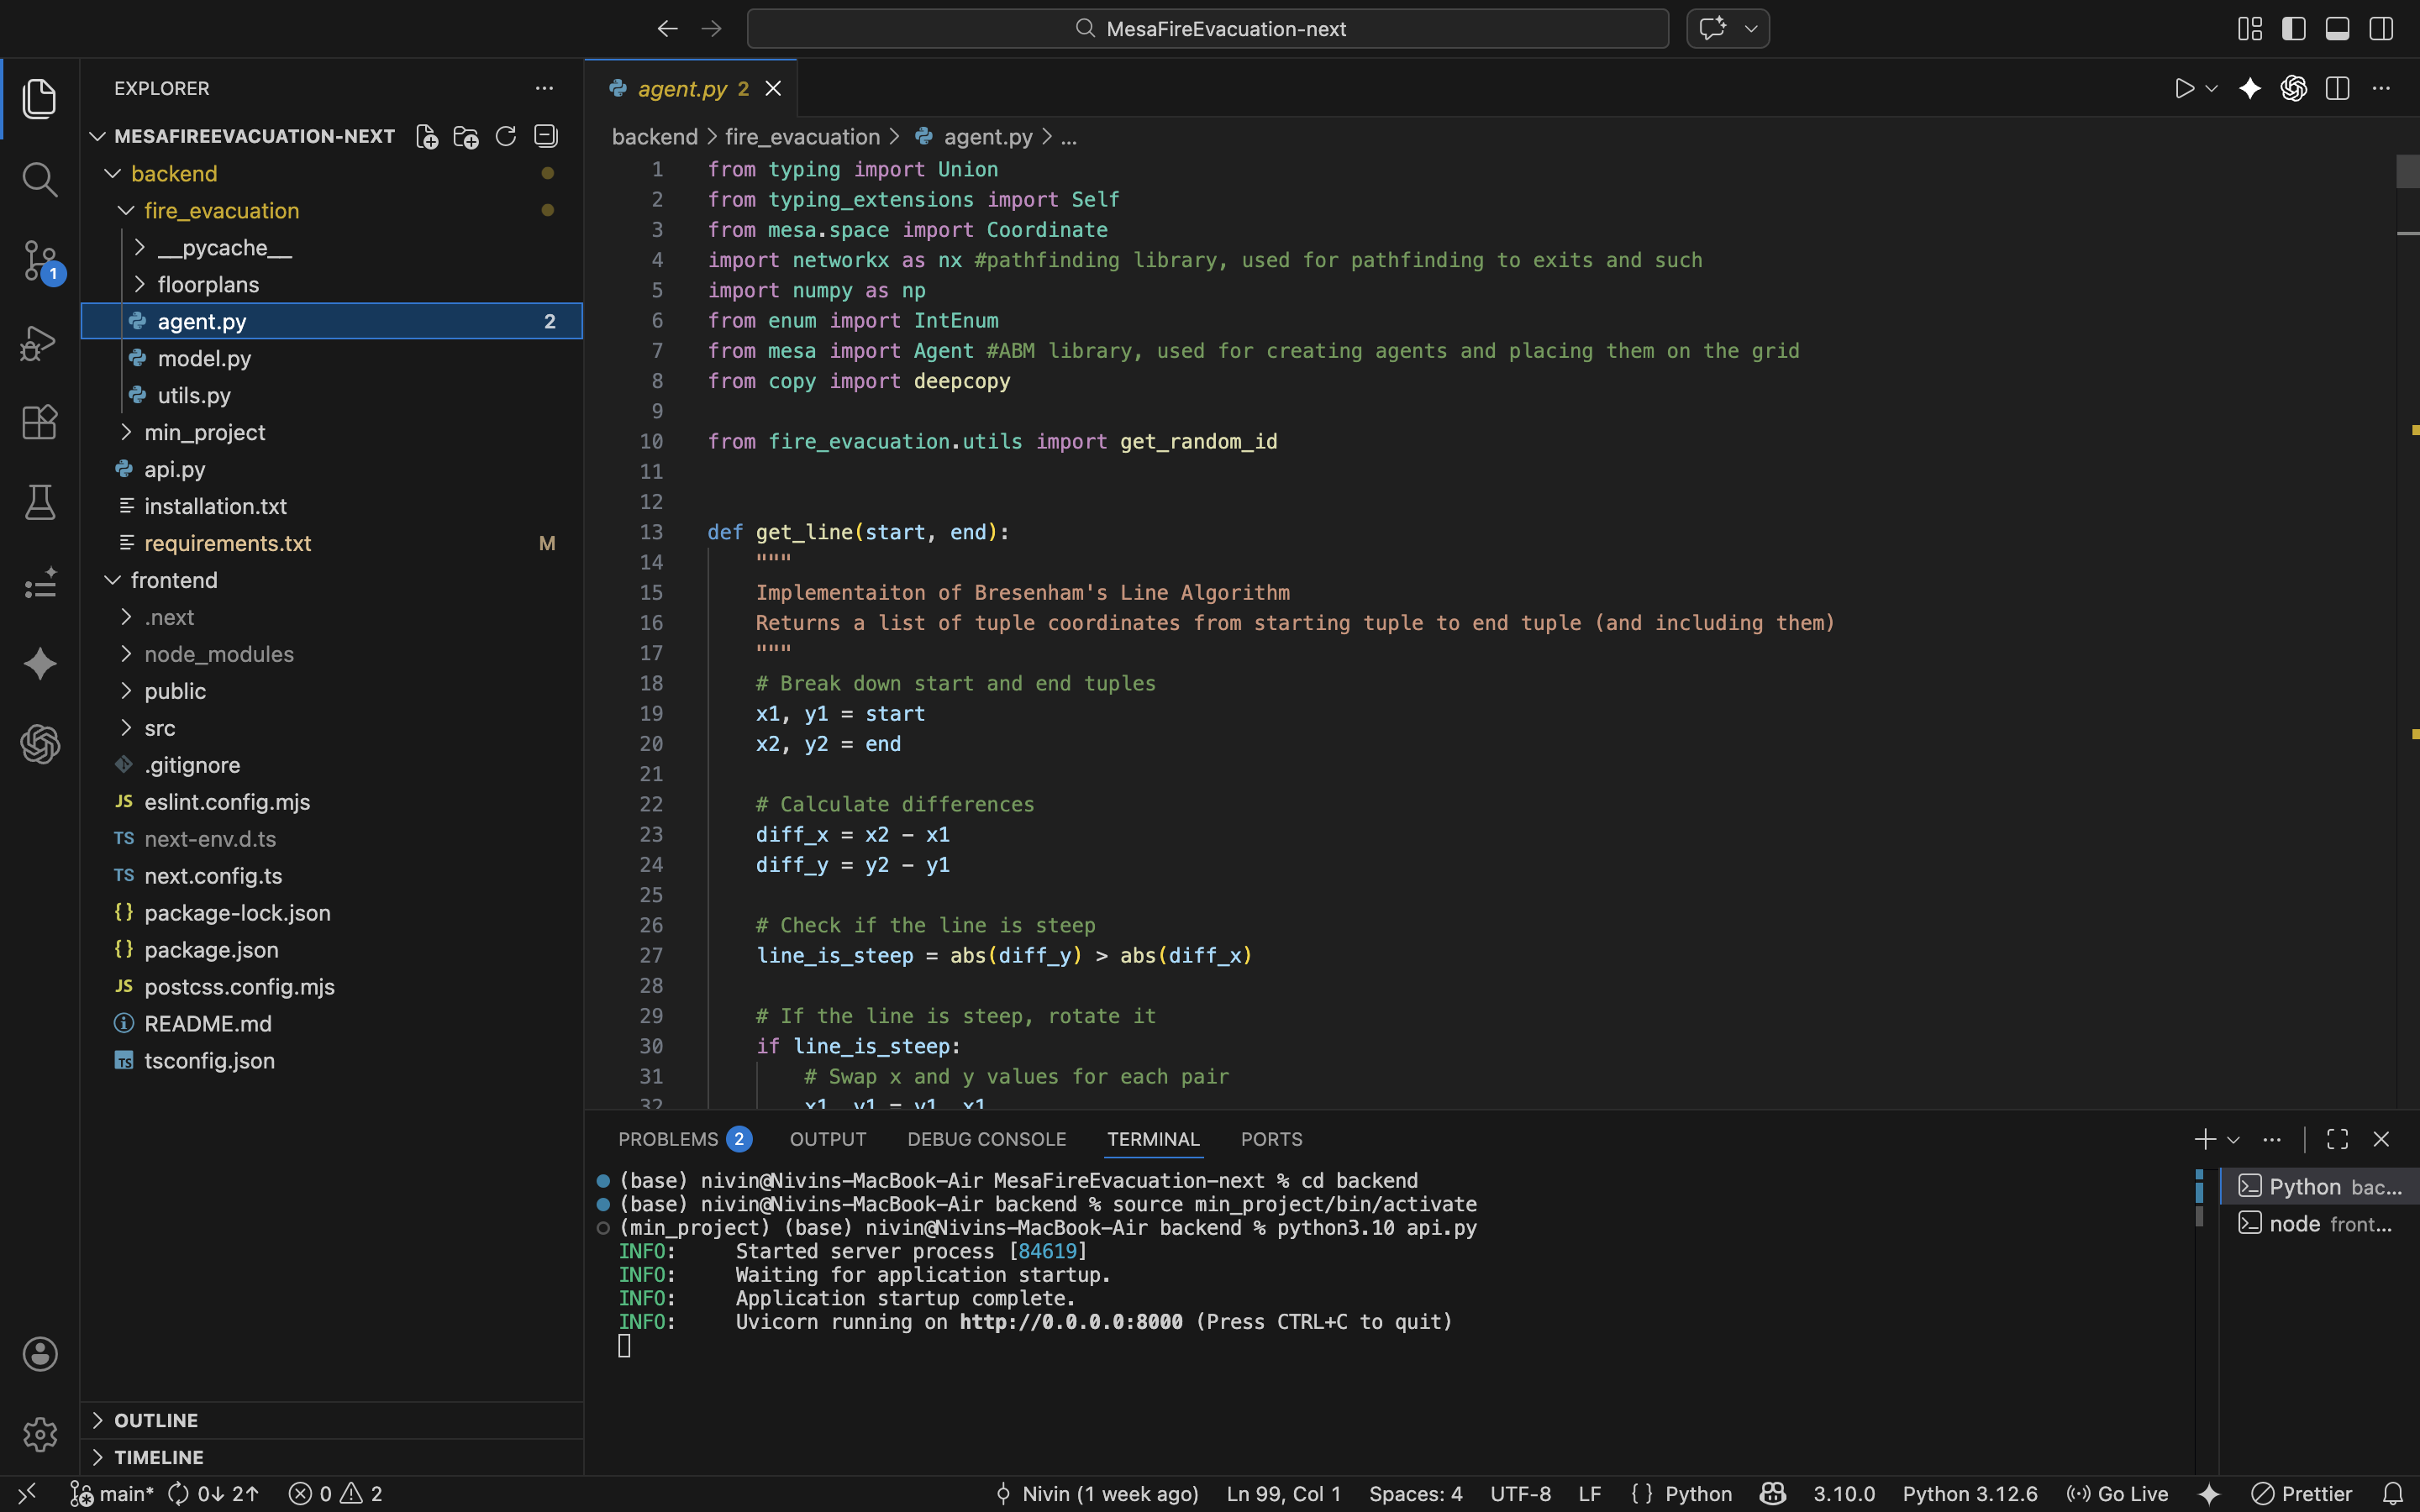
\includegraphics[width=0.8\textwidth, keepaspectratio]{agent.png}
\end{center}
\end{frame}

\begin{frame}
\frametitle{Code Snippet}
\footnotesize 

\begin{center}
    \textbf{api.py} \\
    (FastAPI Implementation) \\
    \vspace{0.2cm}
    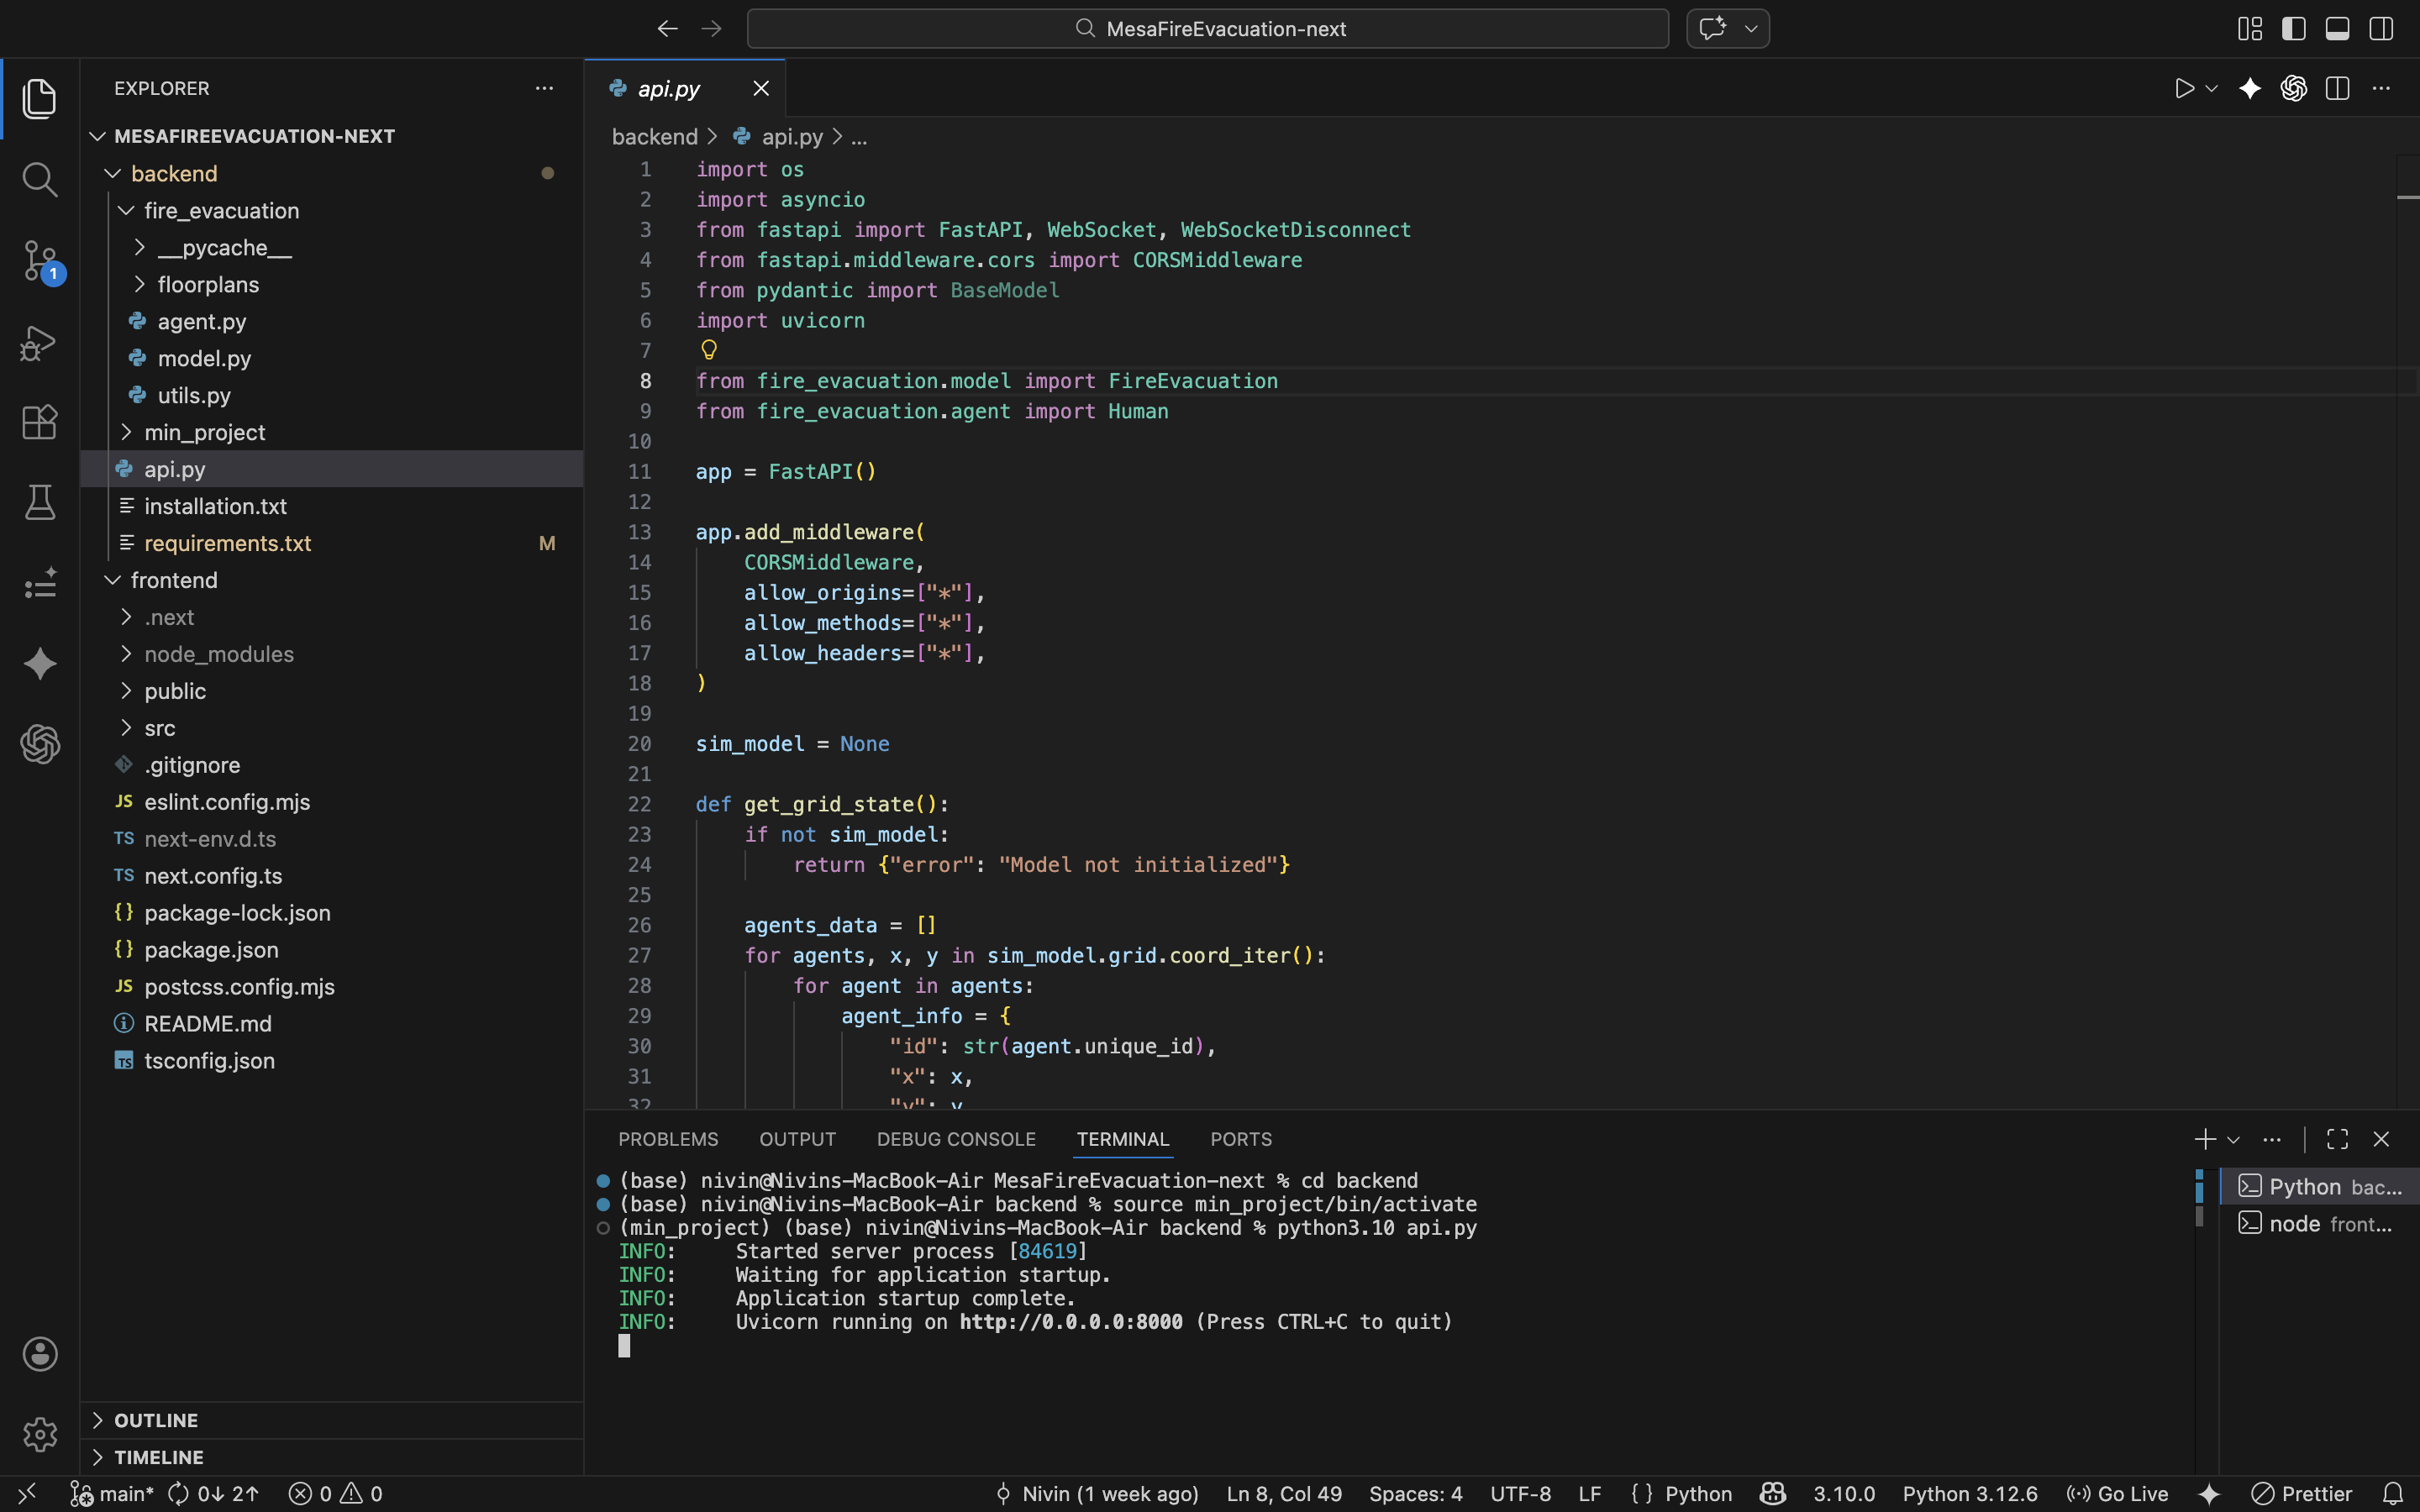
\includegraphics[width=0.8\textwidth, keepaspectratio]{api.png}
\end{center}
\end{frame}

\begin{frame}
\frametitle{Code Snippet}
\footnotesize 

\begin{center}
    \textbf{Floorplans} \\
    (Given as Text Files) \\
    \vspace{0.2cm}
    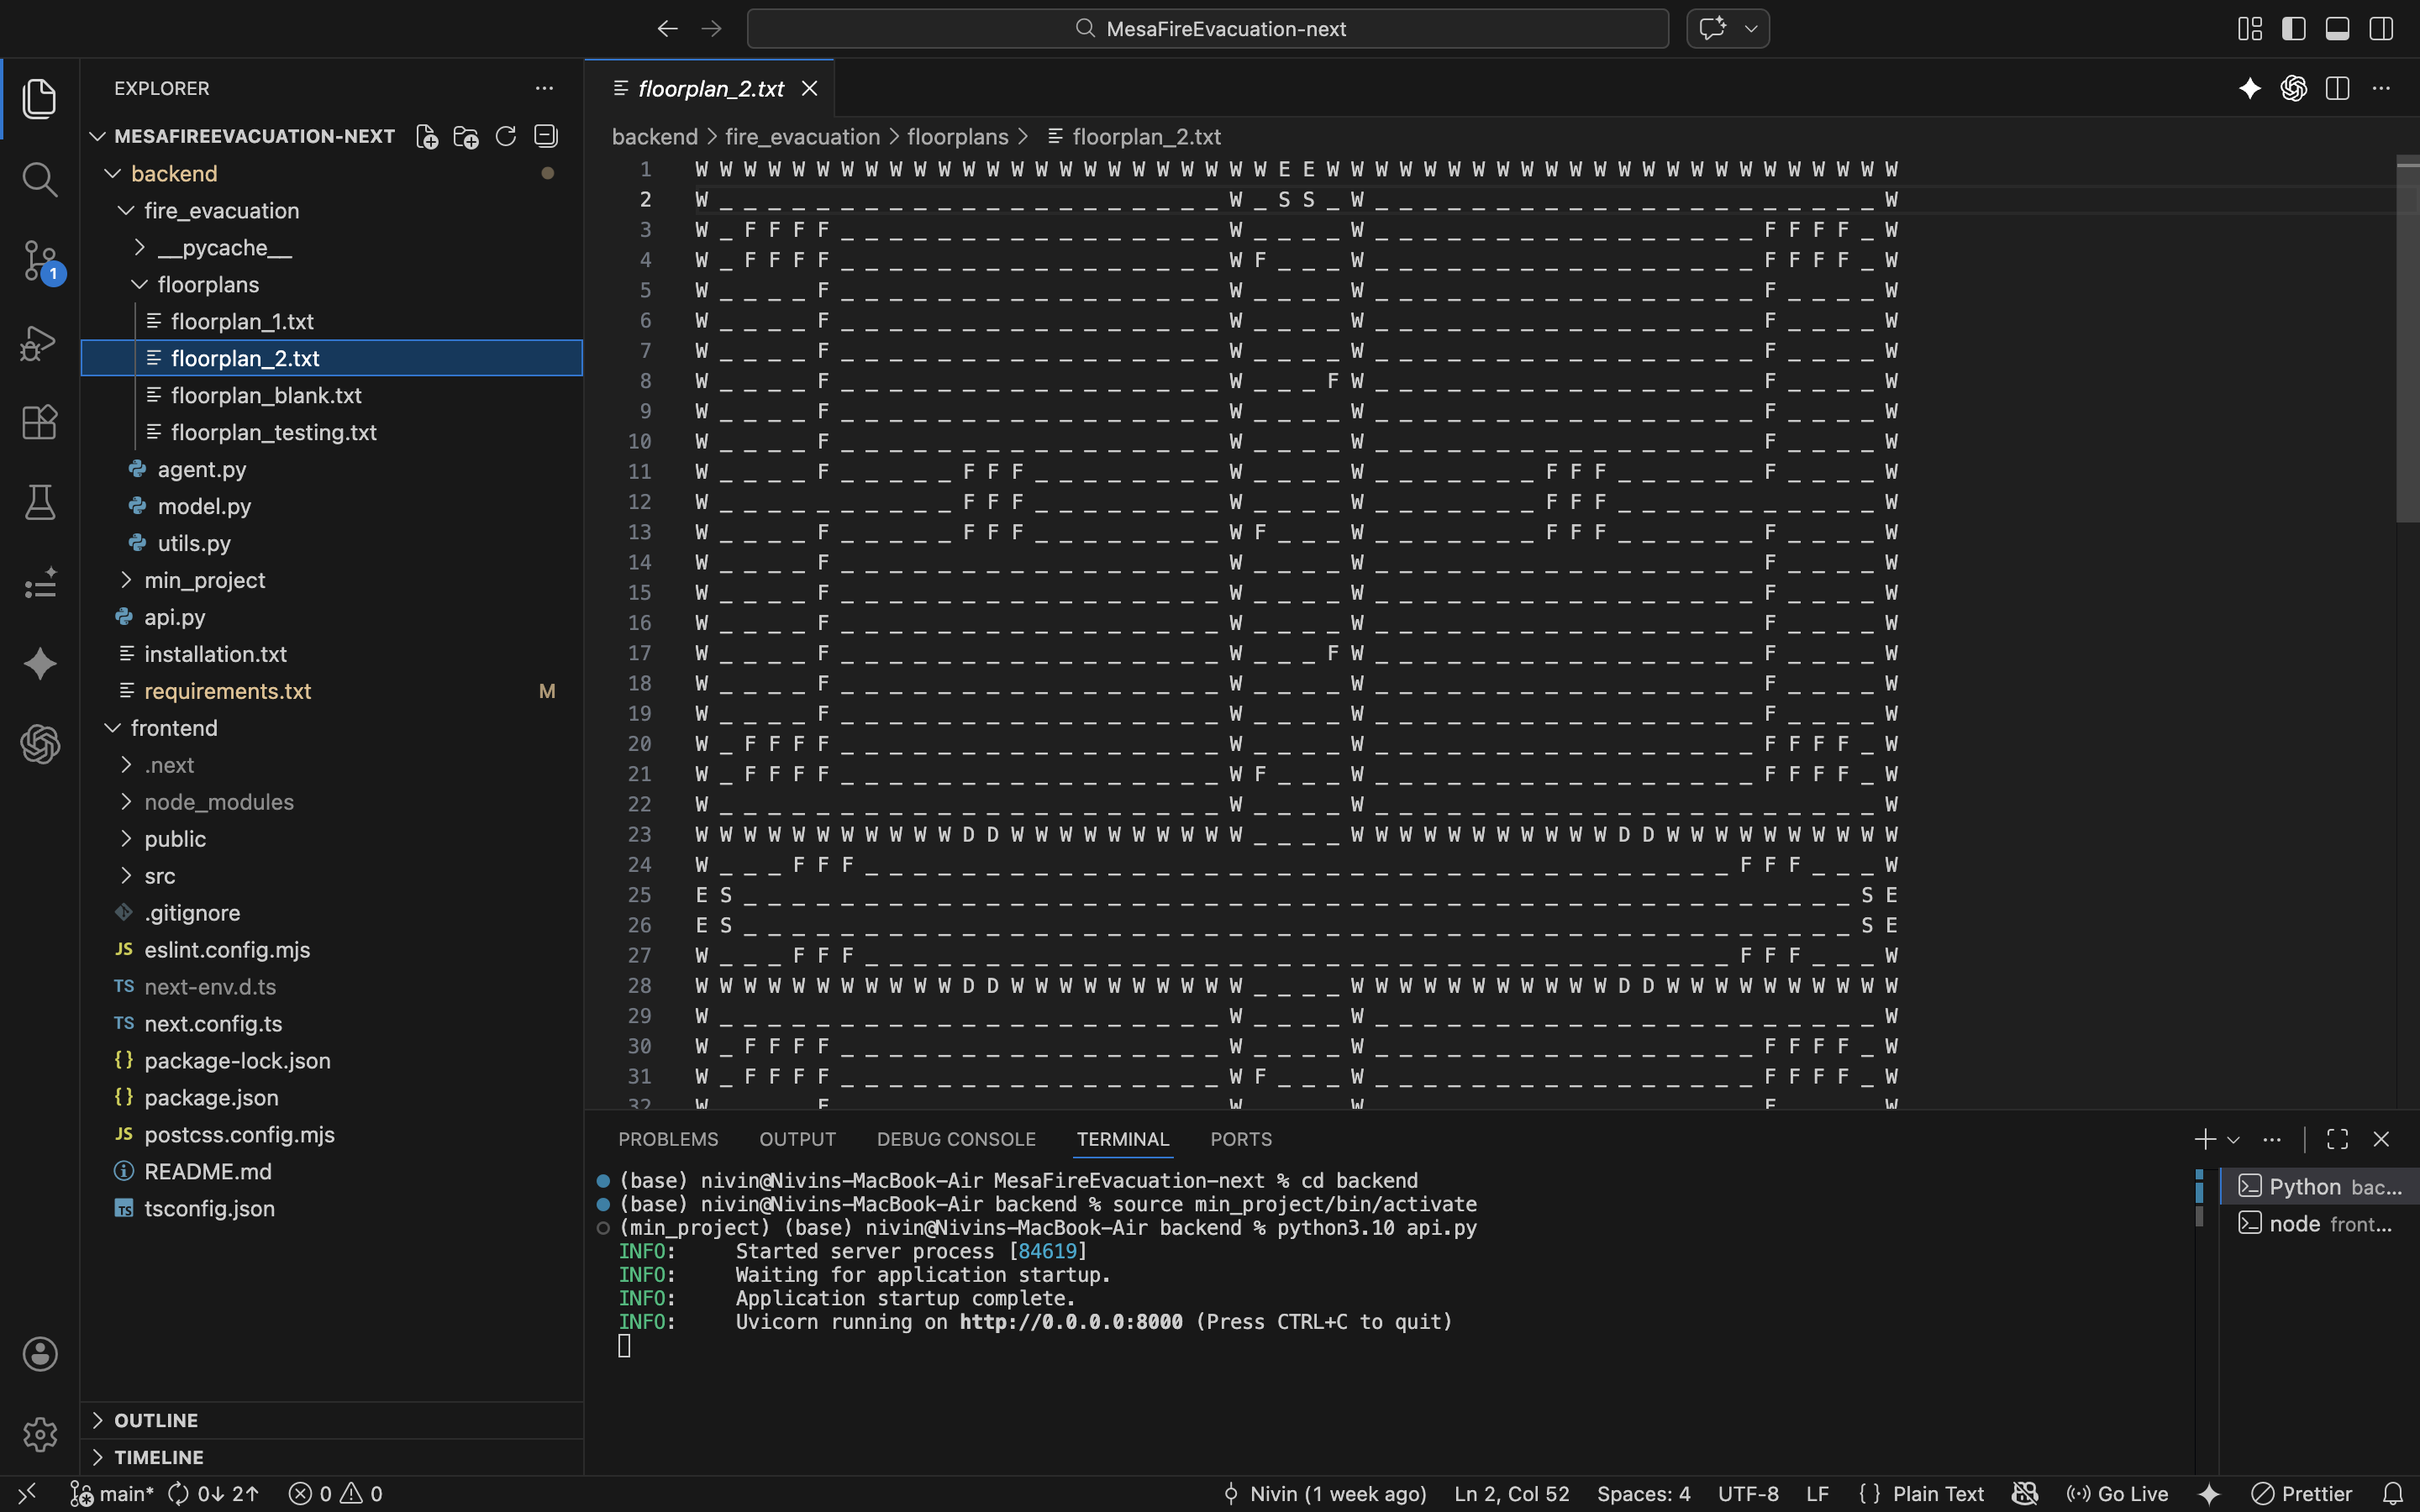
\includegraphics[width=0.8\textwidth, keepaspectratio]{floorplan.png}
\end{center}
\end{frame}

\begin{frame}
\frametitle{Code Snippet}
\footnotesize 

\begin{center}
    \textbf{Frontend} \\
    (Web application design and controls) \\
    \vspace{0.2cm}
    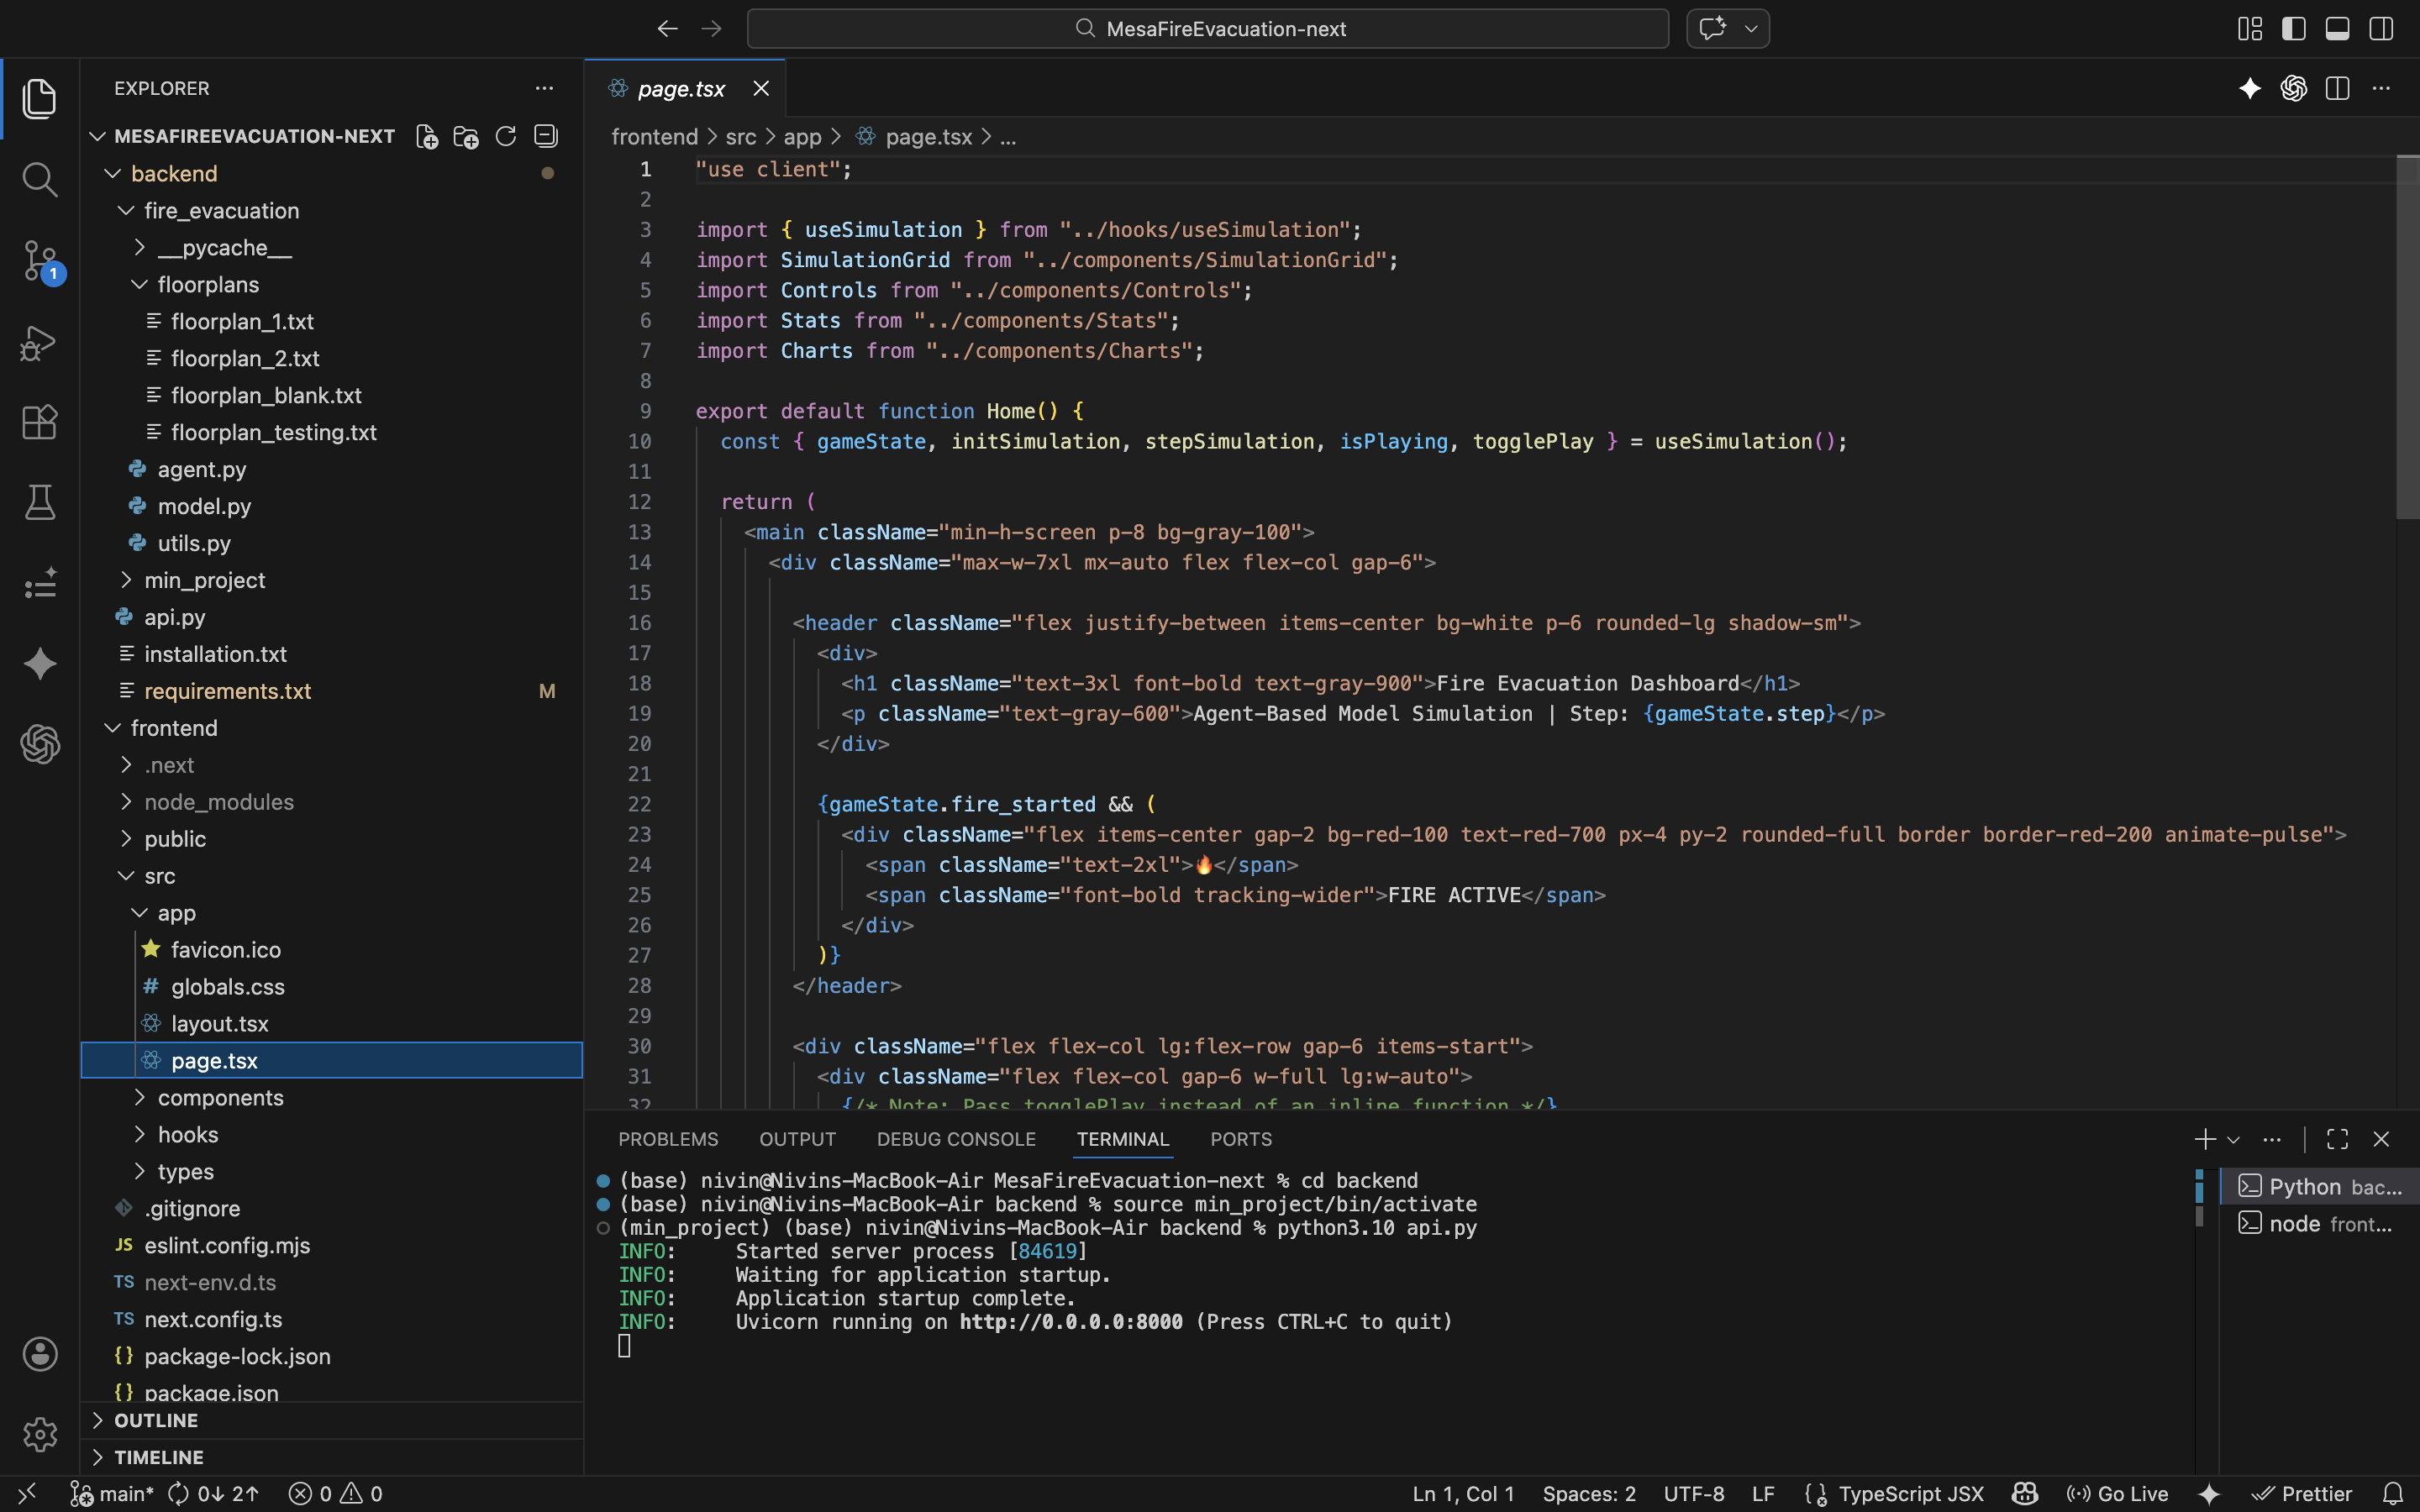
\includegraphics[width=0.8\textwidth, keepaspectratio]{frontend.png}
\end{center}
\end{frame}

\begin{frame}
\frametitle{Application }
\footnotesize 

\begin{center}
    \textbf{Dashboard} \\
    \vspace{0.2cm}
    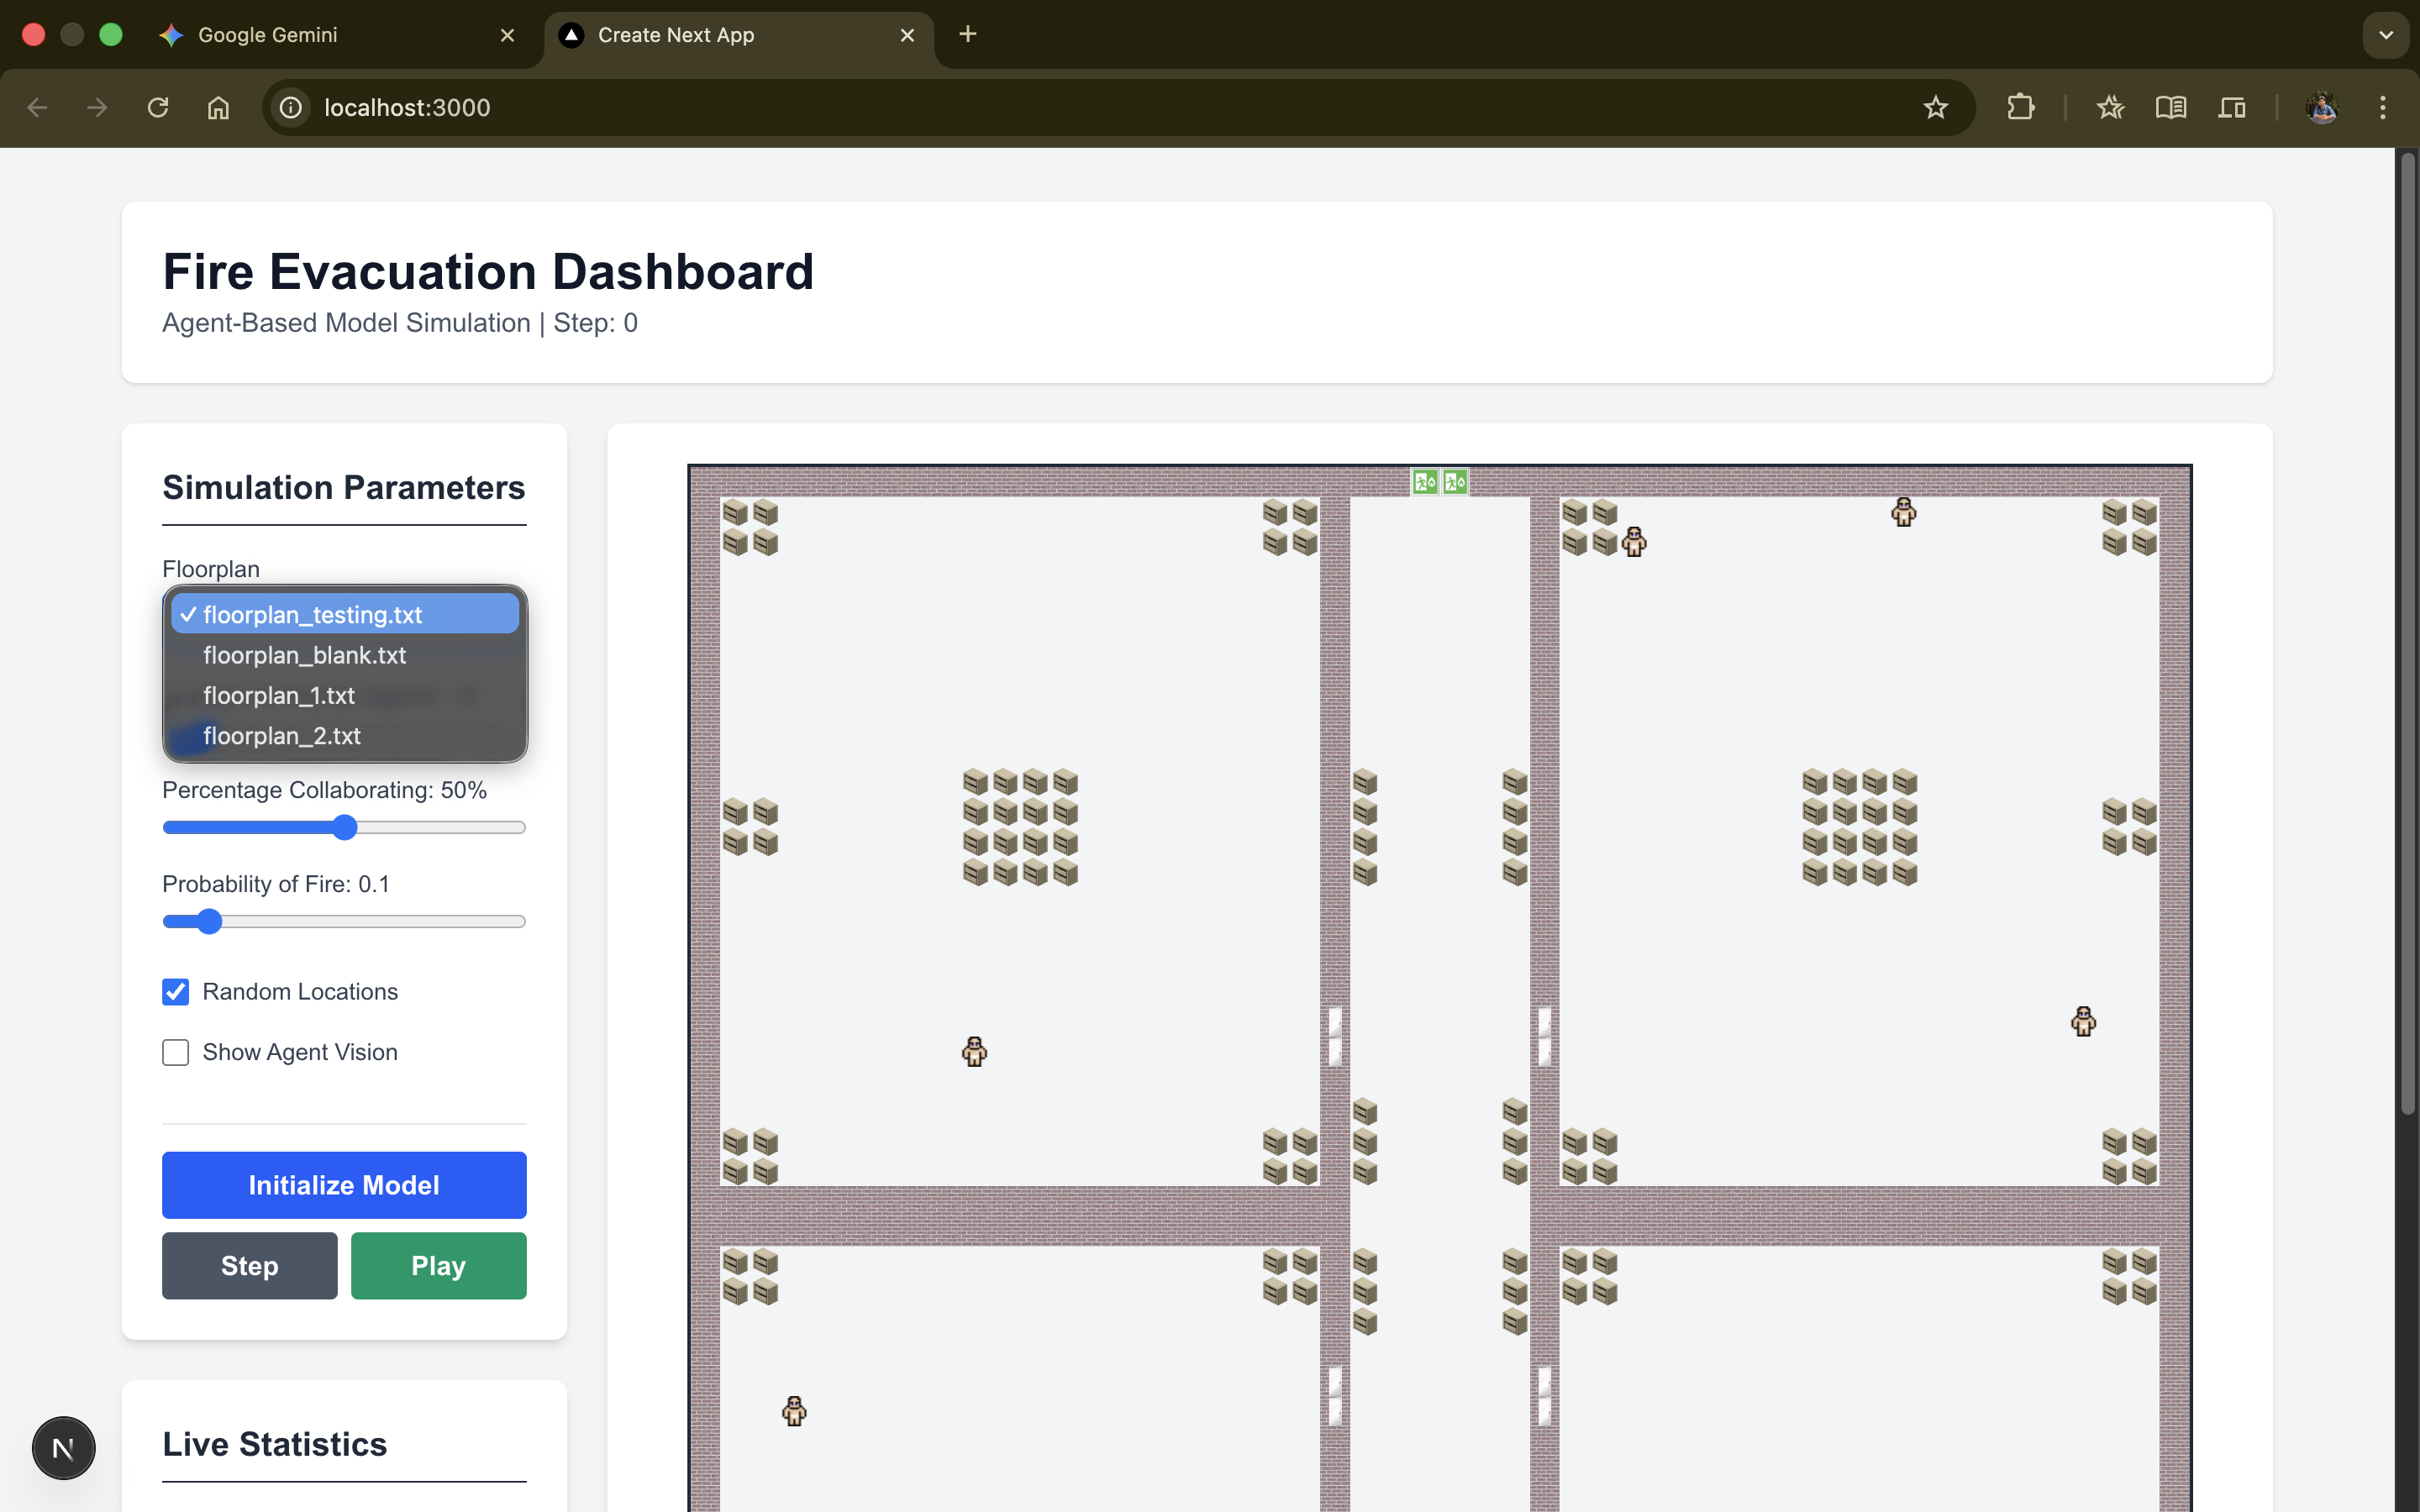
\includegraphics[width=0.8\textwidth, keepaspectratio]{intialization.png}
\end{center}

\end{frame}

\begin{frame}
\frametitle{Application }
\footnotesize 

\begin{center}
    \textbf{Fire Scenario} \\
    \vspace{0.2cm}
    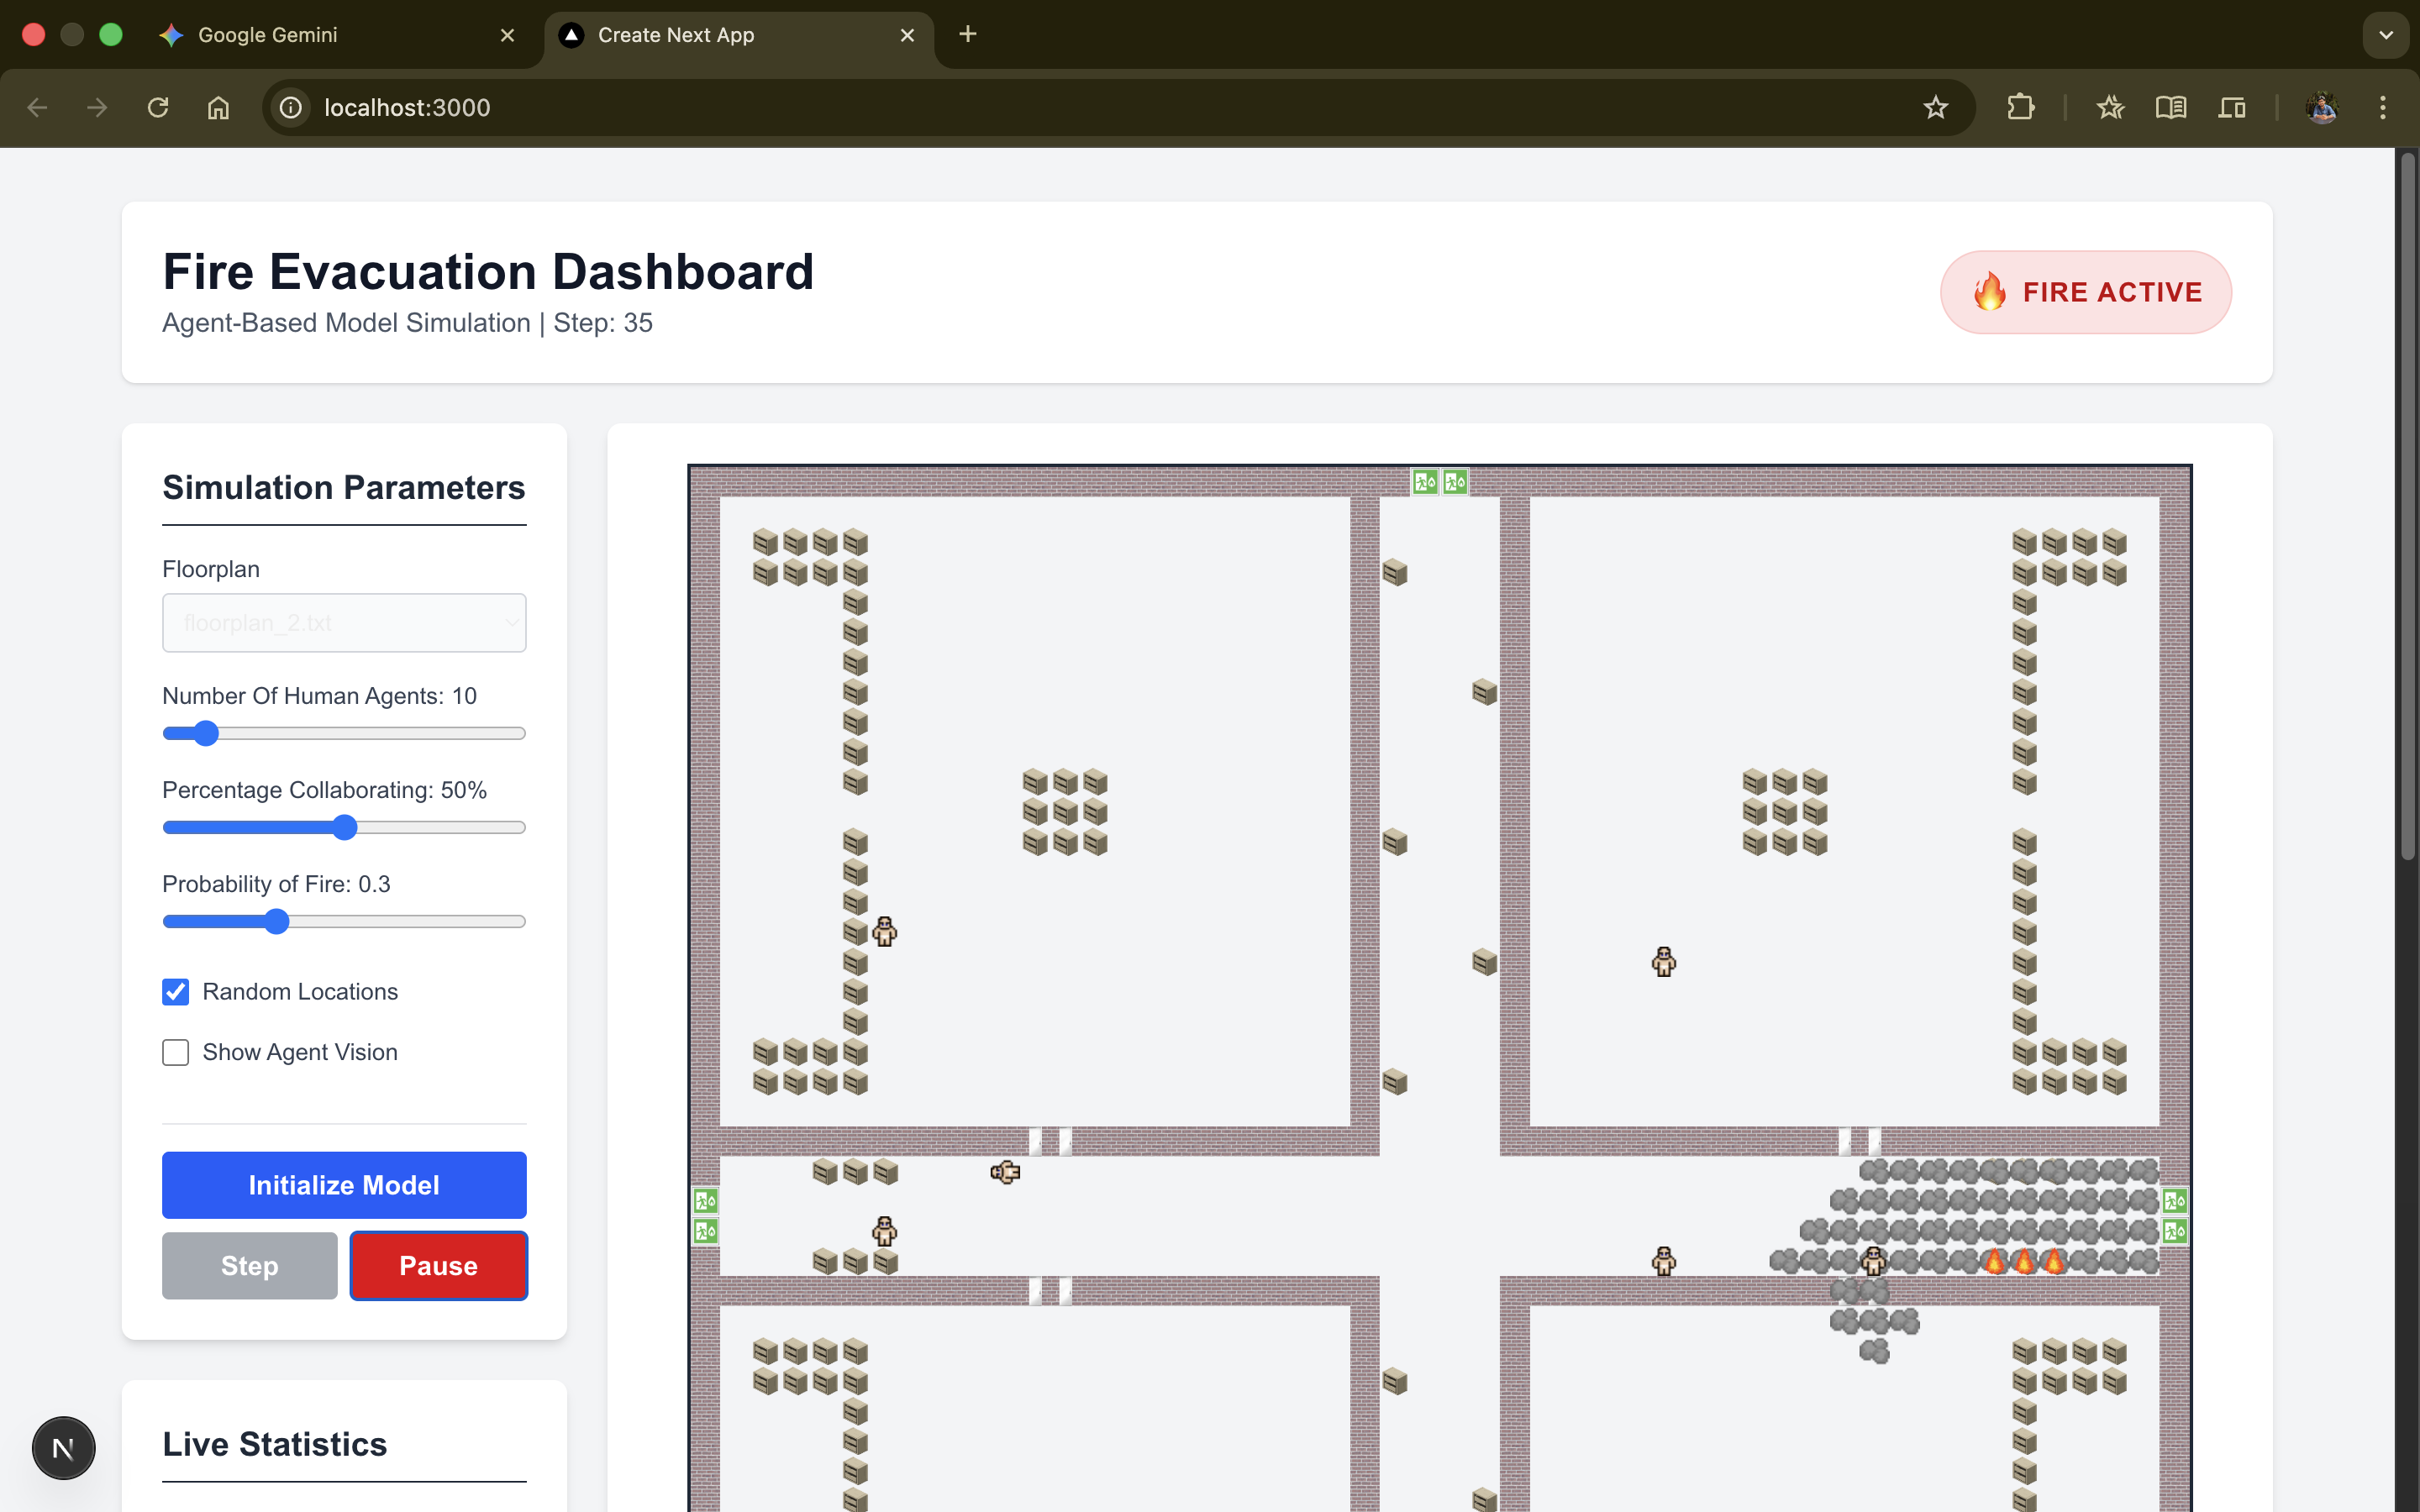
\includegraphics[width=0.8\textwidth, keepaspectratio]{fire.png}
\end{center}

\end{frame}

\begin{frame}
\frametitle{Application }
\footnotesize 

\begin{center}
    \textbf{Statistics} \\
    \vspace{0.2cm}
    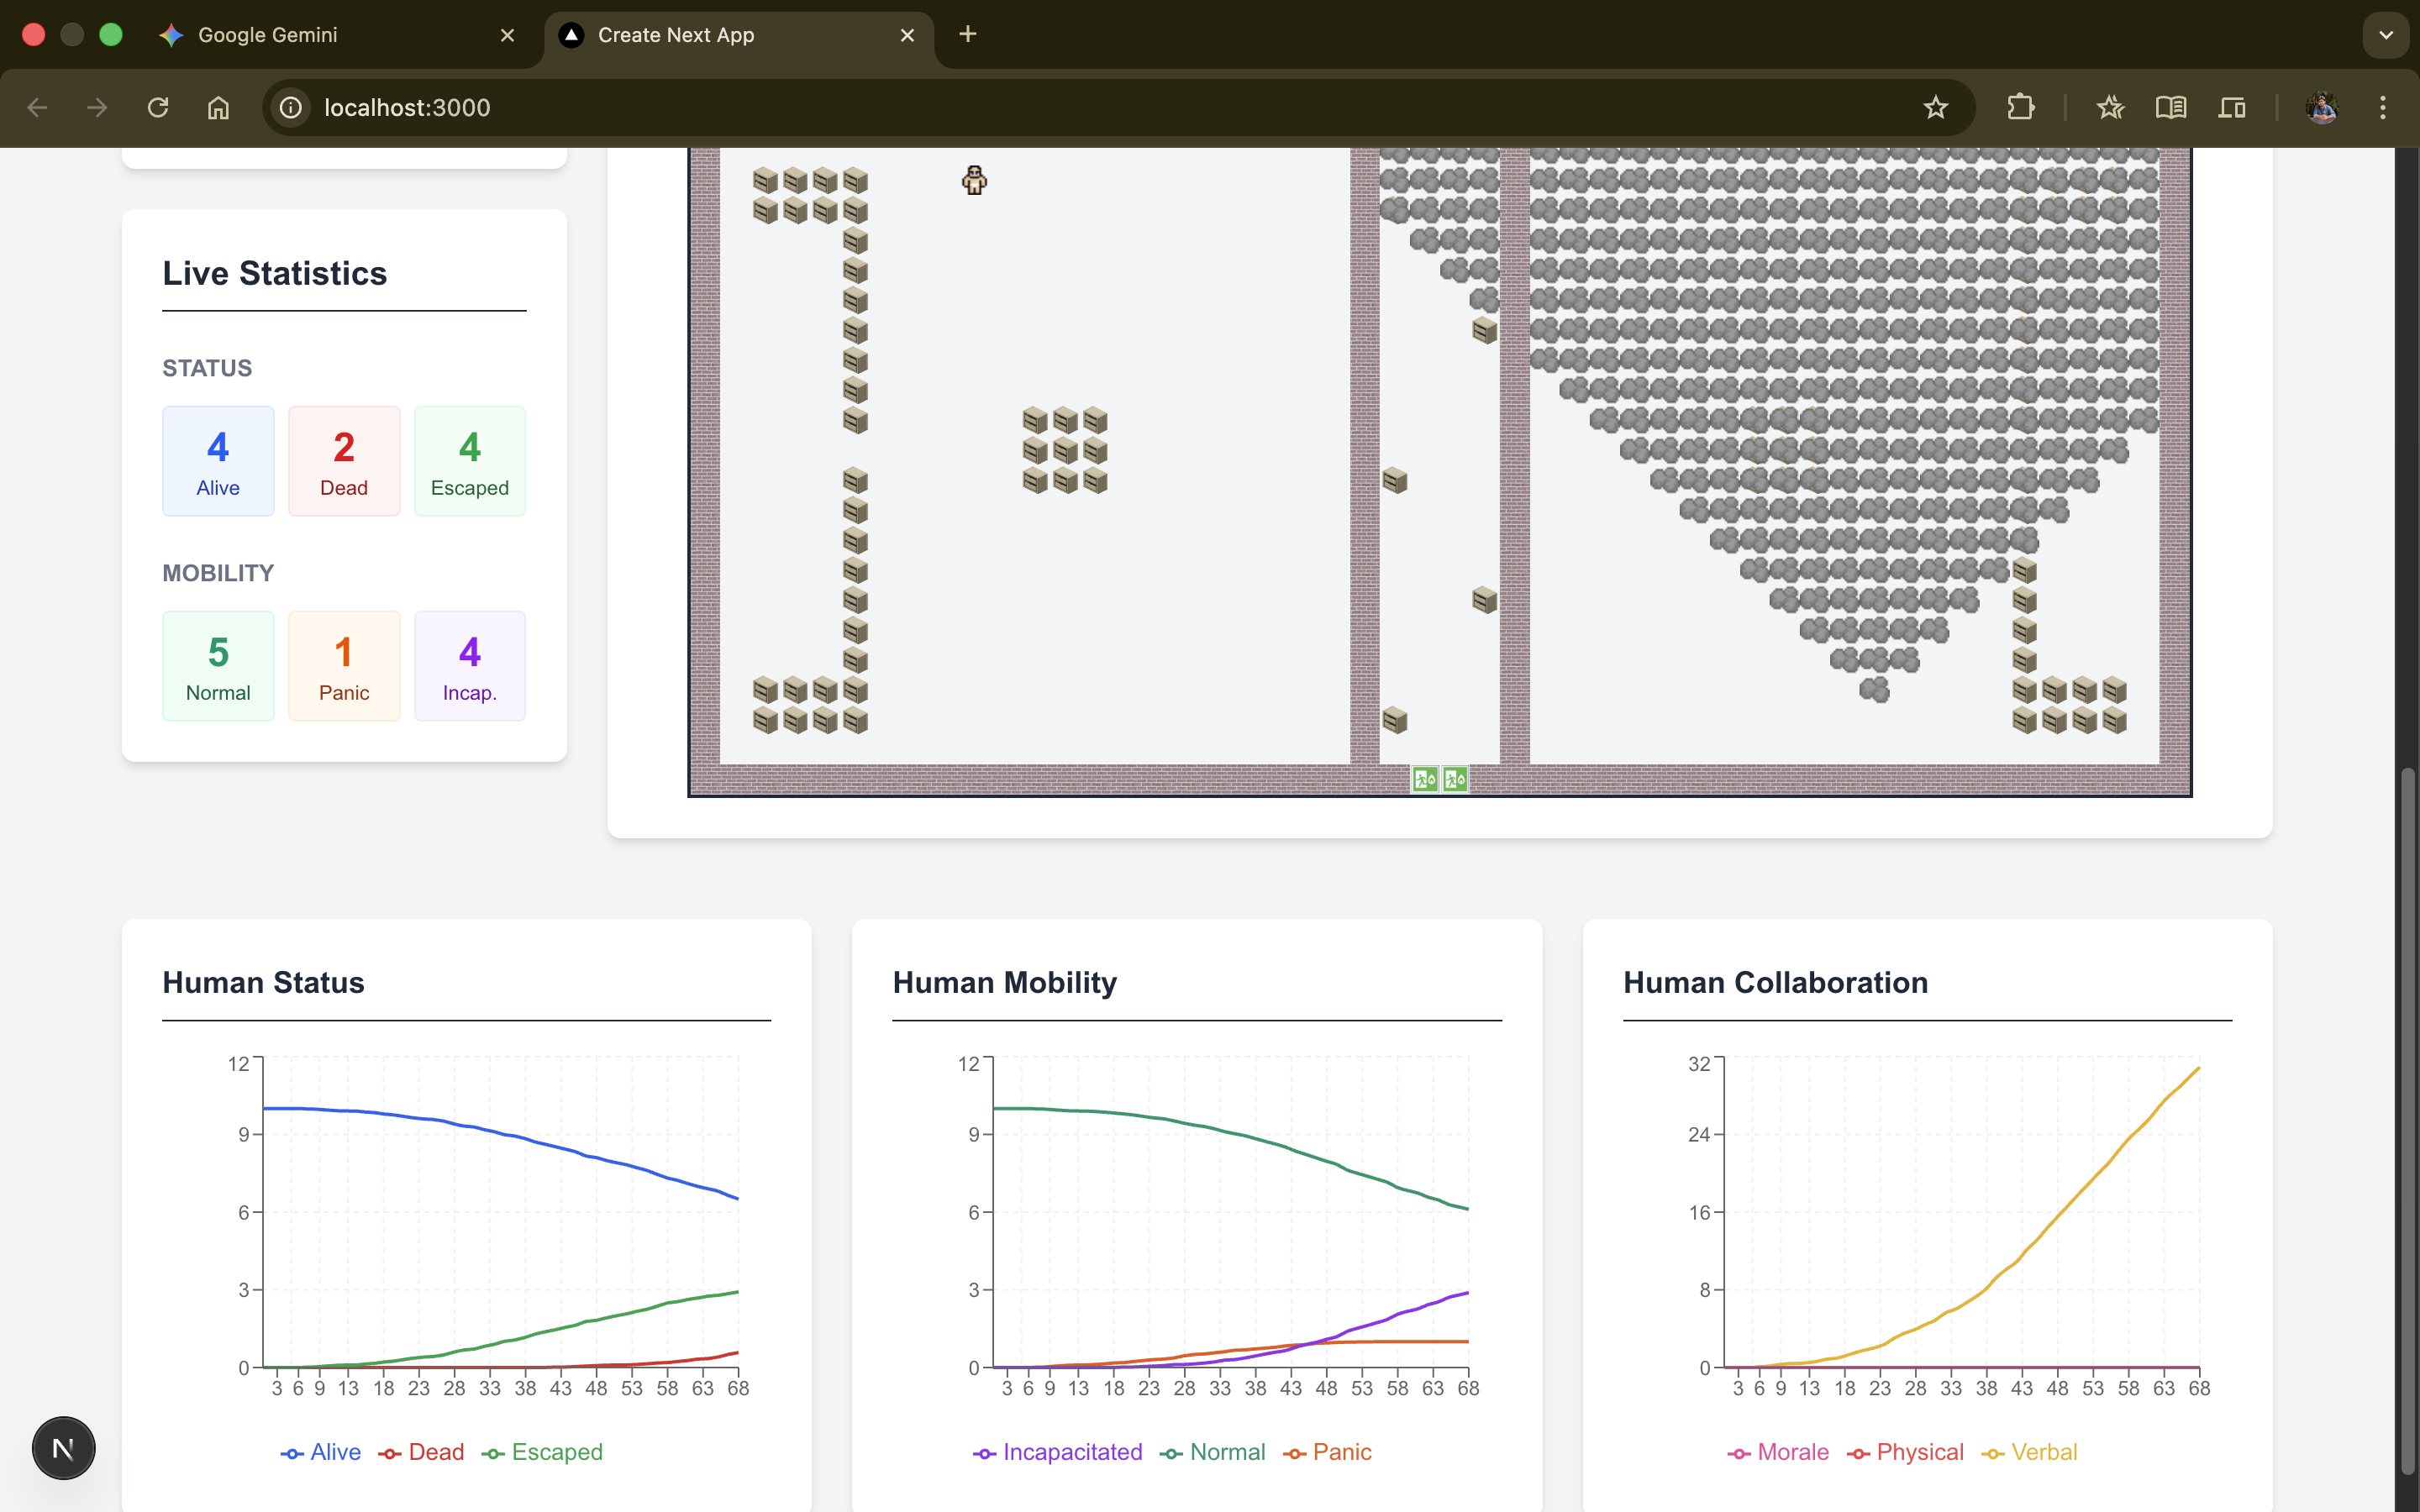
\includegraphics[width=0.8\textwidth, keepaspectratio]{statistics.png}
\end{center}

\end{frame}

%---------------------------------------------------------
% Section: Challenges Faced
%---------------------------------------------------------
\section{Challenges Faced}

\begin{frame}
\frametitle{Challenges Faced}
\textbf{Technical \& Architectural Hurdles} 
\footnotesize 

\begin{itemize}
    \item \textbf{Decoupling the Architecture:} Moving from Mesa's built-in, tightly coupled Tornado server to a modern FastAPI/Next.js stack required completely rewriting the state management and rendering pipeline.
    \item \textbf{Real-Time State Synchronization:} Initial Problem: HTTP polling (fetching data every 500ms) caused UI stuttering and high server overhead. Solution: Implemented persistent WebSockets and CSS \texttt{transition-all} properties to ensure smooth, client-side interpolation of agent movements.
    \item \textbf{Edge-Case Exception Handling:} Encountered critical backend crashes during map initialization (e.g., \texttt{numpy.random.choice} throwing a 500 Internal Server Error on empty floorplans). Solution: Implemented robust fallback logic to safely abort fire spawning if no flammable furniture (F tiles) was present in the custom user array.
\end{itemize}
\end{frame}

\begin{frame}
\frametitle{Challenges Faced}
\textbf{Simulation \& Logic} 
\footnotesize 

\begin{itemize}
    \item \textbf{Computational Overhead of Pathfinding:} Calculating \texttt{networkx.shortest\_path} for dozens of agents simultaneously on every single tick is highly CPU-intensive, especially as the graph dynamically changes due to fire/smoke.
    \item \textbf{Balancing the "Ecosystem":} Tuning the mathematical weights for panic scoring, health degradation, and smoke spread rate. Goal: Ensuring emergent behavior felt realistic (e.g., humans escaping, some panicking) rather than completely chaotic or too easy.
    \item \textbf{Ray-Casting Complexity:} Implementing Bresenham's line algorithm for line-of-sight required careful condition handling to ensure vision was strictly blocked by walls while only being partially obscured by smoke density.
\end{itemize}
\end{frame}

%---------------------------------------------------------
% Section: Future Scope
%---------------------------------------------------------
\section{Future Scope}

\begin{frame}
\frametitle{Future Scope}
\textbf{Advanced Crowd Dynamics} \\
\vspace{0.2cm}
\footnotesize 

\begin{itemize}
    \item \textbf{Stampede Prevention Modeling:} Upgrading the movement logic to include agent-based crowd simulation specifically focused on bottleneck density and stampede prevention at choke points (e.g., stairwells, narrow doors).
    \item \textbf{Crush Mechanics:} Introducing health penalties for agents trapped in highly dense, panicked clusters to accurately reflect the physical dangers of crowd crushes.
    \item \textbf{Dynamic Danger Routing:} Implementing dynamic edge-weighting in the NetworkX graph. As smoke spreads, the "cost" of traveling through those nodes increases, forcing agents to calculate entirely new, safer routes on the fly rather than just stopping.
\end{itemize}
\end{frame}

\begin{frame}
\frametitle{Future Scope}
\textbf{Platform Expansion \& Inclusivity} \\
\vspace{0.2cm}
\footnotesize 

\begin{itemize}
    \item \textbf{Persistent Cloud Storage:} Integrating a production database (e.g., PostgreSQL or MongoDB) to permanently save and share user-generated floorplans from the interactive builder, replacing the ephemeral local \texttt{.txt} file system.
    \item \textbf{Inclusive Agent Modeling:} Introducing diverse agent profiles with varying physical mobilities or cognitive processing speeds to test how inclusive and accessible a building's emergency layout truly is.
    \item \textbf{Explainable AI (XAI) UI:} Adding an interactive frontend feature where clicking an individual agent reveals a real-time log of their internal decision-making process (e.g., "Route A blocked by fire $\rightarrow$ Recalculating $\rightarrow$ Assisting fainted peer").
\end{itemize}
\end{frame}


%---------------------------------------------------------
% Section: Reference
%---------------------------------------------------------
\section{Reference}
\begin{frame}[allowframebreaks]
\frametitle{References}
\scriptsize % Sets a smaller font size for the reference list

\begin{enumerate}
    \item \textbf{Enhancing Building Evacuation Efficiency in Case of Fire Breakout by Integrating Evacuee Categorization Into an Agent-Based Simulation}\\
    \url{https://ieeexplore.ieee.org/document/10820974}
    
    \item \textbf{RESCUE: Crowd Evacuation Simulation via Controlling SDM-United Characters}\\
    \url{https://arxiv.org/pdf/2507.20117}
    
    \item \textbf{An implementation architecture for crowd network simulations}\\
    \url{https://ieeexplore.ieee.org/document/9826689}
    
    \item \textbf{Estimate Crowd Flow Including Side-Trip Behavior When Exiting From Large-Scale Event Venues}\\
    \url{https://ieeexplore.ieee.org/document/11123809}
    
    \item \textbf{Modelling Mass Crowd Using Discrete Event Simulation: A Case Study of Integrated Tawaf and Sayee Rituals During Hajj}\\
    \url{https://ieeexplore.ieee.org/document/9439797}
    
    \item \textbf{CrowdAR Table: An AR system for Real-time Interactive Crowd Simulation}\\
    \url{https://ieeexplore.ieee.org/document/9319072}
    
    \item \textbf{Coordinating dynamic signage for evacuation guidance: A multi-agent reinforcement learning approach integrating mesoscopic crowd modeling and fire propagation}\\
    \url{https://www.sciencedirect.com/science/article/abs/pii/S0960077925002590}
    
    \item \textbf{Toward an Integrated Intelligent Framework for Crowd Control and Management (IICCM)}\\
    \url{https://ieeexplore.ieee.org/document/10942376}
\end{enumerate}

\end{frame}

\end{document}
